%%%%%%%%%%%%%%%%%%%%%%%%%%%%%%%%%%%%%%%%%%%%%%%%%%%%%%%%%%%%%%%%%%%%%%%%%%%%%%%%
%%%                               80 COLONNES                                %%%
%%%%%%%%%%%%%%%%%%%%%%%%%%%%%%%%%%%%%%%%%%%%%%%%%%%%%%%%%%%%%%%%%%%%%%%%%%%%%%%%

\chapter{Analyse critique de l'état de l'art}
\label{ChEtatArt}

Nos travaux ont, d'un point de vue pratique, principalement concerné les
couches basses des piles réseau de systèmes d'exploitation spécialisés
pour les réseaux de capteurs sans-fil. Ces réseaux fonctionnent à l'heure
actuelle principalement avec le protocole IEEE 802.15.4
\cite{IEEE802154-2011}, même si l'utilisation de technologies alternatives
(tel le BLE~--- \lang{Bluetooth Low Energy} également appelé
\lang{Bluetooth Smart}) commence à émerger.

Notre objectif était de réaliser et d'améliorer l'implantation logicielle
de la couche MAC (\lang{Medium Access Control}, protocole d'accès au médium,
en l'occurence le canal radio 802.15.4 voulu). Pour des raisons techniques
évidentes, nous avons également été amenés à travailler sur la couche PHY
logicielle sous-jacente (consistant en les pilotes des émetteurs~/
récepteurs radio des appareils concernés), ainsi que sur l'interface
entre ces deux couches.

Le présent chapitre va ainsi s'articuler en 3 sections~:
\begin{itemize}
\item la première va brièvement rappeler les bases du protocole IEEE 802.15.4,
dont la couche physique a servi de base à tous nos travaux~;
\item la seconde résumera les différentes familles et technologies des
protocoles MAC applicables aux réseaux 802.15.4~;
\item quant à la troisième et dernière, elle reprendra les différents
systèmes d'exploitation spécialisés dans les systèmes embarqués et notamment
dans les réseaux de capteurs sans-fil. Cette troisième section sera plus
analytique et critique, et s'intéressera particulièrement aux fonctions
offertes par ces systèmes aux programmeurs, tout spécialement pour le
développement des couches bases des piles réseau.
\end{itemize}

Aucune de ces sections ne prétend à l'exhaustivité, mais cherche à donner
les données nécessaires et suffisantes pour comprendre les bases à partir
desquelles nous avons effectué nos travaux.

%%%%%%%%%%%%%%%%%%%%%%%%%%%%%%%%%%%%%%%%%%%%%%%%%%%%%%%%%%%%%%%%%%%%%%%%%%%%%

\section{Le protocole IEEE 802.15.4}
\label{SecProto802154}

Le standard IEEE 802.15.4 définit les couches basses (PHYsique et MAC)
de réseaux sans-fil destinés à relier des appareils sur une très faible
distance et avec un faible débit (on parle de LR-WPAN~: \lang{Low-Rate
Wireless Personal Area Network}, en contrepartie d'une consommation
d'énergie très modeste.

Apparu dans sa première version en 2003, il a été révisé en 2006 puis en
2011, et complété par divers amendements (802.15.4a, 4b, 4c, 4d et 
à l'heure actuelle 4e).

Ce standard ne définissant que les deux couches les plus basses de la pile
réseau, il est le plus souvent utilisé de concert avec d'autres protocoles
définissant les couches hautes. On peut notamment utiliser des piles
protocolaires basées sur IP (\lang{Internet Protocol})~--- telle que 6LoWPAN
\cite{6LoWPAN}~--- ou non~--- comme ZigBee.
Toutes ces piles réseau reposent ainsi sur le standard 802.15.4.

La figure \vref{FigCompar802154IPOSI} résume de façon schématique la
comparaison entre le standard IEEE 802.15.4, et les deux piles de protocoles
réseaux complètes et couramment utilisées que sont le modèle OSI et le
modèle Internet (souvent appelé abusivement <<~TCP/IP~>>).

\begin{figure}[!hbt]
\centering
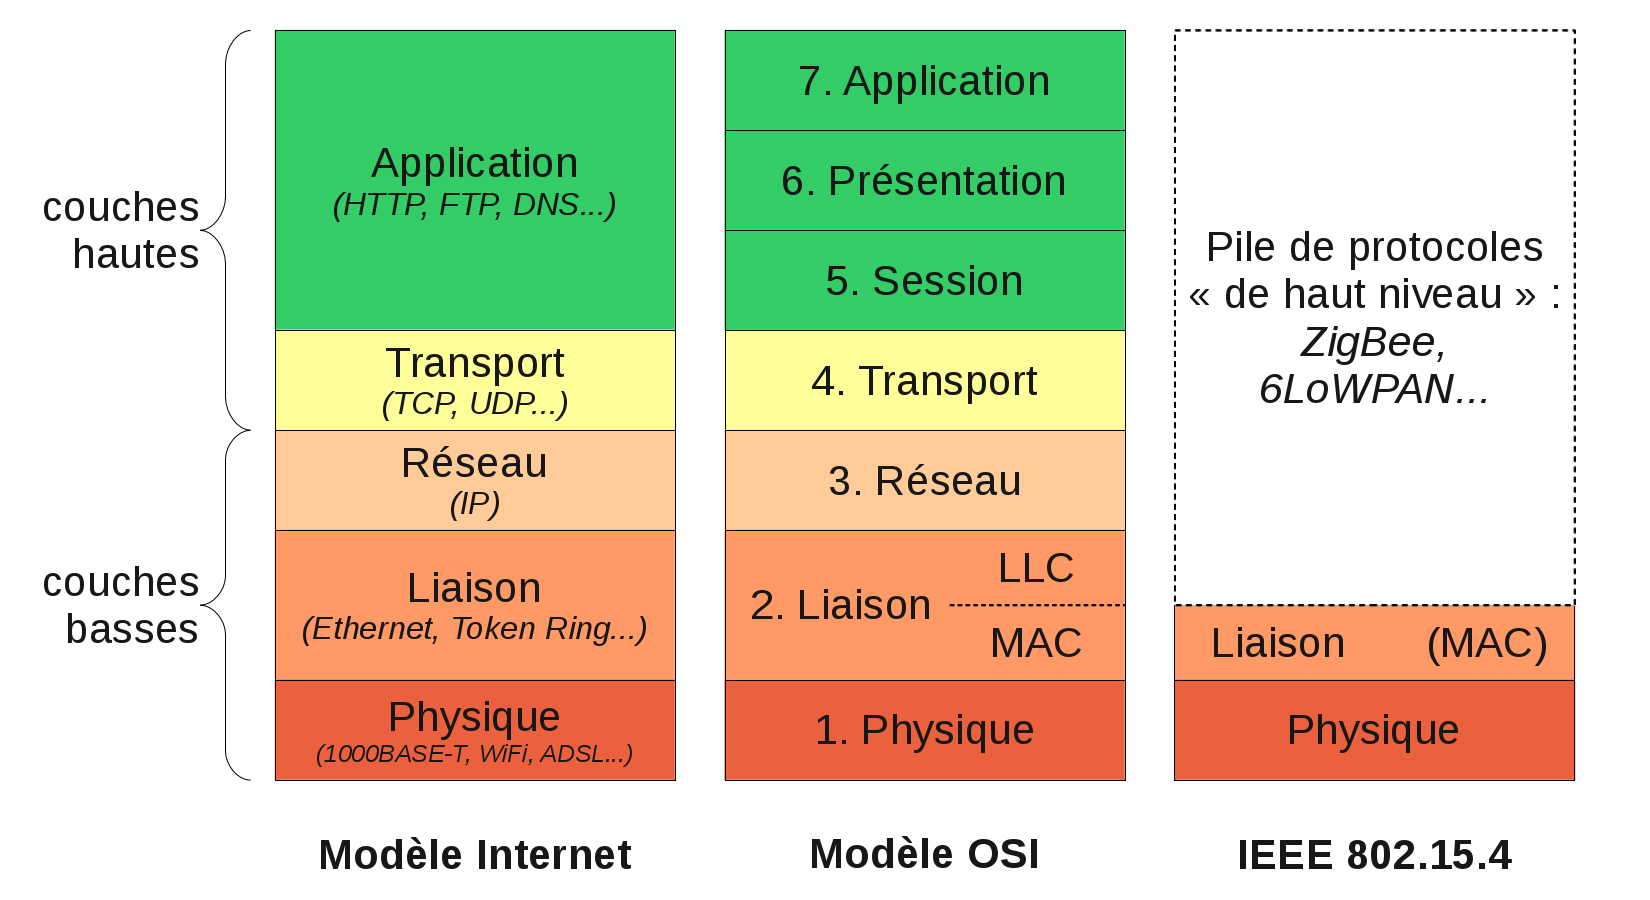
\includegraphics[width=12.5cm]{images/ch3-ip-vs-osi-vs-802154.png}
\flcaption{Comparaison entre la pile 802.15.4 et les piles OSI et Internet.}
\label{FigCompar802154IPOSI}
\end{figure}


\subsection{Couche physique}
\label{Subsec802154PHY}

La couche physique (PHY) 802.15.4 offre les fonctionnalités suivantes~:

\begin{description}

\item[Bandes de fréquences.]
De base, le standard offre trois bandes~:
une fréquence (canal) unique à 868~MHz disponible en Europe~;
une bande autour de 915~MHz offrant d'abord 10 canaux (puis étendue à 30)
disponible en Amérique du Nord~;
et la bande ISM de 2,4~GHz offrant 16 canaux et disponible dans le monde
entier.

À l'origine (2003), seule la bande à 2,4 GHz permettait d'atteindre le
débit maximal de 250~kbps, les basses fréquences (868 et 915~MHz) étaient
elles limitées à de faibles débits (20 à 40~kbps) en contrepartie d'une
portée plus grande (due à un moindre affaiblissement).
Le choix d'une bande de fréquence correspondait ainsi à un compromis entre
débit et portée, en sus d'un choix dicté par des considérations géographiques.

La révision de 2006, grâce à l'introduction de nouvelles méthodes de
modulation du signal radio, a permis aux bandes à 868 et 915~MHz d'atteindre
des débits de 100 et 250~kbps. Le choix d'une bande radio dépend donc
désormais surtout du déploiement géographique envisagé pour les réseaux
considérés.

En outre, les différents amendements ont ajouté de nouvelles bandes
de fréquences disponibles (315, 430 et 780~MHz disponibles en Chine~;
950~MHz disponible au Japon).
Ces mêmes amendements apportèrent également des méthodes de modulation
de signal supplémentaires, permettant notamment l'utilisation de bandes
à très hautes fréquences (jusqu'à 10 GHz).

L'amendement 802.15.4a a égalemement ajouté la notion d'\lang{Ultra-Wide
Band} (UWB), lequel offre, outre de plus hauts débits, la possibilité de
mesurer notamment précisément les temps de vol (c-à-d. les délais de
communication entre deux noeuds).

Les différents émetteurs~/ récepteurs radio (RF) à la norme 802.15.4 ne
peuvent pas fonctionner sur toutes les fréquences du standard~: leur choix
dépend donc de la bande de fréquences souhaitée.
Parmi les plus utilisés à l'heure actuelle, on peut par exemple citer~:
\begin{itemize}
\item La famille Texas Instruments (TI) ChipCon (CC) 1000/1100. Cette famille
regroupe des émetteurs~/ récepteurs pour les bandes à 868 et 915 MHz.
\item La famille TI CC 2400/2500, regroupant des émetteurs~/ récepteurs pour
la bande à 2,4 GHz.
\item La famille Atmel AT86RF230, regroupant également des émetteurs~/
récepteurs pour la bande à 2,4 GHz.
\end{itemize}
Nous avons au cours de nos travaux utilisé des appareils dotés de
composants radio appartenant aux deux dernières familles citées (CC2420
et AT86RF231/233), et fonctionnant donc sur la seule bande ISM à 2,4 GHz.

Notons également que l'on trouve de plus en plus fréquemment des
microcontrôleurs intégrant directement un émetteur~/ récepteur radio
dans la même puce~: par exemple, le STM32W108 de ST Microelectronics,
le SAMR21 ou la famille ATmegaRFR2 \cite{DSATmegaRFR2} d'Atmel.

\item[Mode de liaison.]
Le couche physique du standard IEEE 802.15.4 est une \emph{liaison
half-duplex}. Cela signifie que si la communication entre deux appareils
à la norme IEEE 802.15.4 est bien \emph{bidirectionnelle}~--- chaque
appareil peut assumer le rôle d'émetteur \emph{et} celui de récepteur~---
il est \emph{impossible à une seule radio au standard IEEE 802.15.4 d'émettre
et de recevoir simultanément}. La transmission d'informations entre deux
\lang{motes} dans les réseaux de capteurs sans-fil se fait donc \emph{de
façon alternée}, chaque noeud pouvant à chaque instant donné soit émettre,
soit recevoir des données~; mais jamais les deux en même temps (si le
noeud ne possède qu'un seul émetteur~/ récepteur radio).

L'un des rôles majeurs de la couche directement supérieure (MAC) est
justement de déterminer à quels instants la radio doit être en mode émission,
et à quels autres instants en réception~--- et aussi éventuellement à quels
instants elle est désactivée (pour économiser de l'énergie).

Notons que ce fonctionnement \emph{half-duplex} n'est pas propre à ce
standard 802.15.4. Le standard IEEE 802.11 (plus connu sous le nom de
\lang{``WiFi''}) est lui aussi un standard \lang{half-duplex}. Ce mode
de fonctionnement est en fait mieux adapté aux communications sans-fil,
utilisant le médium radio, lequel est par nature sujet à la diffusion,
aux variations rapides d'état et à d'autres facteurs nuisant à la qualité
de transmission. (Les réseaux câblés sont la plupart du temps en
\lang{full-duplex}, c-à-d. peuvent transmettre et recevoir simultanément,
généralement en consacrant~--- au moins~--- un fil à chaque sens
de communication.)

Ce mode de fonctionnement \lang{half-duplex} a des conséquences pratiques~:
un émetteur~/ récepteur radio doit régulièrement passer du mode émission
au mode réception et inversement. Une telle procédure n'est pas instantanée,
chaque puce radio ayant un délai de retournement indiqué dans sa
\lang{datasheet}. Le standard IEEE 802.15.4~--- dans sa version de 2011~---
indique un délai maximal pour passer du mode émission au mode réception et
inversement, que toutes les radios conformes au standard ne sont pas censées
dépasser~: constante \emph{aTurnaroundTime}, égale à 12 symboles (soit
192~$\mu$sec. pour la plupart des puces radio émettant sur la bande
de 2,4 GHz).

\item[Format de trames.]
Le standard définit un format~--- très simple~--- de trame physique
(\lang{``frame''}), dont la taille est limitée à 127 octets.
Ces 127 octets incluant les entêtes des couches supérieures (dont la
couche MAC), la taille disponible pour les données proprement dites
(charge utile ou \lang{``payload''}) est en général nettement inférieure.

\item[Modes d'adressage.]
Deux modes d'adressage complémentaires sont pris en charge~:
\begin{itemize}
\item un adressage court sur 16~bits (plus un identifiant de réseau~---
identifiant PAN~--- de 16~bits également) dont l'intérêt est de limiter
la taille des entêtes de trames~;
\item un adressage long (dit <<~adressage IEEE~>>) sur 64~bits permettant
\lang{a priori} directement une identification unique de chaque appareil.
\end{itemize}

\item[Détection du médium.]
Le standard inclut la détection d'énergie (ED~: \lang{Energy Detection})
sur le médium radio, et par extension la vérification de la disponibilité
du canal radio (CCA~: \lang{Clear Channel Assessment}).

\item[Qualité de service.]
Le standard prend en charge la définition et l'indication de la qualité
de liaison (LQI~: \lang{Link Quality Indicator}) pour une transmission
de trame donnée. Le RSSI (\lang{Received Signal Strength Indicator}),
s'il n'est quévoqué dans le glossaire du standard 802.15.4, est également
la plupart du temps pris en charge au niveau physique (émetteurs~/
récepteurs radio).

\end{description}

Toutes ces propriétés sont implantées de façon matérielle par les
différents émetteurs~/ récepteurs radio conformes au standard 802.15.4~---
qu'il s'agisse de composants autonomes, ou de circuits intégrés à des
microcontrôleurs ou \lang{System-on-Chip} (SoC).

La couche PHY, au niveau logiciel, notamment dans un système d'exploitation
spécialisé, consiste donc en un jeu de primitives (implantées dans des
pilotes) permettant d'exploiter ces émetteurs~/ récepteurs radio. On peut
envisager cette couche comme une couche d'abstraction matérielle
(HAL~: \lang{Hardware Abstraction Layer}) vis-à-vis de la couche MAC
et des couches supérieures de la pile réseau du système.


\subsection{Couche MAC}
\label{Subsec802154MAC}

Située immédiatement au-dessus de la couche physique, la couche MAC
du standard 802.15.4 repose sur la méthode CSMA/CA (\lang{Carrier Sense
Multiple Access with Collision Avoidance}). Une version différente de
cette technologie est déjà utilisée (sous le même nom) dans le standard
IEEE 802.11 (alias \lang{``WiFi''}).

La couche MAC standard peut utiliser cette méthode selon deux modalités
différentes, selon l'utilisation ou non de \lang{``beacons''} (ou balises
\footnotemark[1]) pour synchroniser les différents noeuds et identifier
les différents réseaux (PAN). Sans \lang{``beacons''}, la couche MAC
standard emploie toujours des cycles de fonctionnement (\lang{``duty
cycles''}) fixes, sans prendre en compte l'utilisation réelle du réseau
et le débit des données transmises. Le mode <<~avec \lang{beacons}~>>
permet d'ajuster certains paramètres de fonctionnement \cite{TheseSKhssibi}.
Certains éléments restent toutefois immuables, même dans ce mode (par
exemple les 16 \lang{slots} de temps dans la \lang{superframe}).

\footnotetext[1]{Pour des raisons pratiques, nous emploierons dans la suite
de ce manuscrit le terme anglo-saxon \lang{``beacon''}, plus utilisé dans
la littérature.}

Le standard 802.15.4 est à la base conçu pour faire fonctionner des réseaux
ayant une topologie en étoile~; pour cela, le standard permet de
différencier les noeuds en deux types~:

\begin{itemize}

\item les noeuds à fonctionnalités complètes (FFD~: \lang{Full Function
Devices}), capables de jouer aussi bien le rôle de <<~noeud simple~>>
occupant une des extrêmités du réseau, que celui plus évolué de coordinateur
de réseau (en mode <<~avec \lang{beacons}~>>)~;

\item les noeuds à fonctionnalités réduites (RFD~: \lang{Reduced Function
Devices}), limités au rôle de <<~noeuds simples~>>

\end{itemize}

Dans notre terminologie, un <<~noeud simple~>> est un noeud dont la
défaillance ne met pas en péril le fonctionnement de l'ensemble,
au contraire d'un routeur ou d'un coordinateur dont la seule panne
entraîne la perte de tout un réseau.

Un exemple de base d'un schéma topologique d'un réseau de capteurs
sans-fil (WSN) est montré figure \vref{FigTopoWSN}. Celui présenté
ici est composé de quatre sous-réseaux (PAN) différents, possédant chacun
un routeur jouant également le rôle de coordinateur de son PAN. Les noeuds
simples (<<~feuilles~>> de l'arborescence) ne communiquent qu'avec leur
propre coordinateur, ces derniers se chargeant de transmettre les données
de PAN en PAN de façon adéquate.

\begin{figure}[!hbt]
\centering
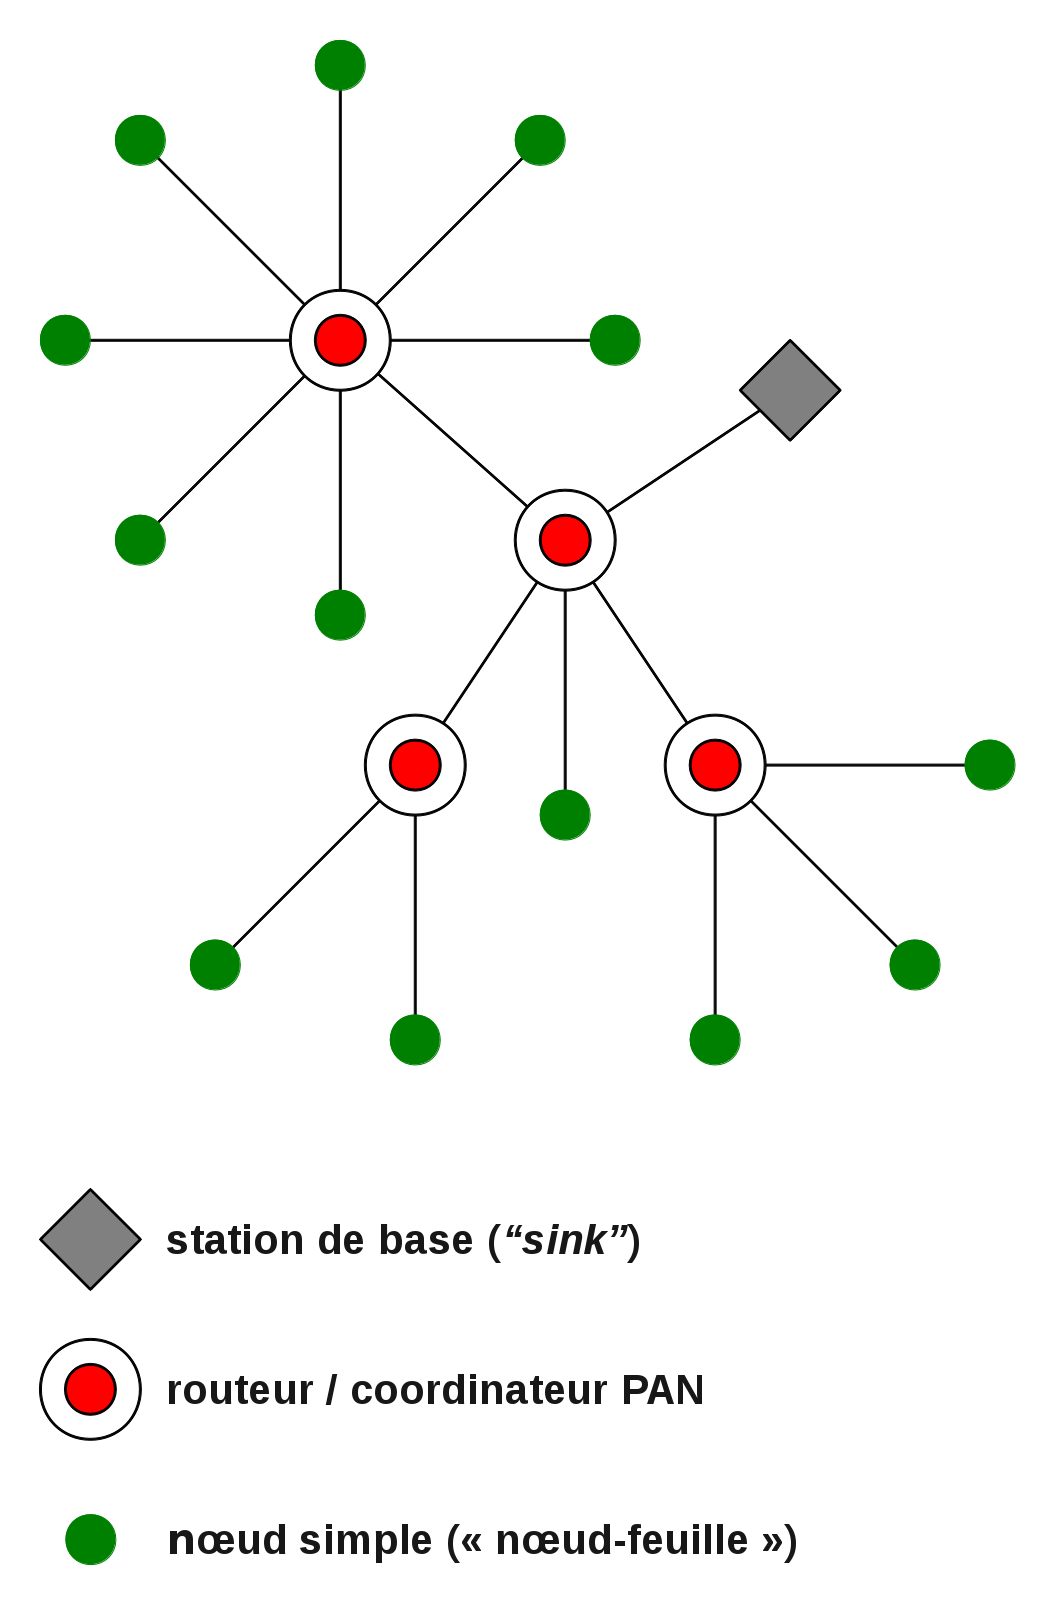
\includegraphics[width=7cm]{images/ch3-topo-wsn.png}
\flcaption{Schéma topologique d'un réseau de capteurs sans-fil (WSN).
(D'après \cite{coursEnsem})}
\label{FigTopoWSN}
\end{figure}

Ces réseaux (PAN) peuvent eux-mêmes être reliés entre eux de façon maillée
et/ou arborescente (selon les protocoles de routage utilisés par dessus
802.15.4).

\subsubsection{CSMA/CA}
\label{ParCSMACA}

Cette méthode consiste à éviter les collisions potentielles sur le médium
en vérifiant préalablement la disponibilité du canal radio et, en cas
d'encombrement, en attendant pendant un délai aléatoire avant de retenter
une écoute.

Plus précisément, l'implantation de CSMA/CA dans le standard 802.15.4
en version de base <<~non slottée~>> est la suivante~:

\begin{enumerate}

\item un noeud souhaitant émettre une trame doit d'abord attendre pendant
un délai dont la durée est \emph{aléatoirement} choisie entre 0 et
$2^{BE} - 1$ unités de temps nommées \nom{BP} (\lang{``Backoff Period''})~.
La valeur d'une BP est une constante dépendant de la bande choisie pour
la couche physique (elle vaut 320~microsecondes pour la bande ISM à 2,4 GHz).
La valeur $BE$ est nommée \lang{``Backoff Exponent''}, et est initialisée
à une valeur définie dans le standard sous le nom de \emph{macMinBE}
(3 par défaut).

\item une procédure de CCA est alors effectuée~: le CCA consiste à écouter
le medium radio durant un délai spécifique~--- nommé DIFS
(\lang{Distributed Inter-Frame Space})~---, si le medium reste libre
pendant ce délai, le noeud peut alors émettre sa trame~; 

\item si le médium radio est encombré, on revient à la première étape
d'attente d'un délai aléatoire, en ayant toutefois incrémenté la valeur
de BE, dans la limite de la valeur maximale \emph{macMaxBE} définie
par le standard (5 par défaut). Toutefois, au bout d'un nombre maximal
d'essais, défini par le standard sous le nom de \emph{macMaxCSMABackoffs}
(4 par défaut), l'envoi de la trame est considéré comme échoué par la
couche MAC.

\end{enumerate}

La méthode CSMA/CA peut également fonctionner en mode <<~slotté~>>, de
façon à s'adapter aux protocoles MAC où les transmissions doivent se caler
sur des intervalles de temps (\lang{``slots''}) bien définis. Dans ce cas,
un nouveau paramètre, nommé \lang{``Contention Window''} (\emph{CW})
intervient pour s'assurer que le médium radio a été détecté libre (CCA)
un certain nombre de fois avant de commencer une émission~; cette étape
supplémentaire a notamment pour but de faciliter la transmission des
messages d'acquittement signalant la bonne réception d'une trame (ACK).
Par défaut, le standard fixe la valeur initiale de $CW$ ($CW_0$) à 2.

L'organigramme décrivant le fonctionnement de la méthode CSMA/CA est
schématisé dans la figure \vref{FigOrganigrammeCSMACA}.
Dans cette figure, la branche de gauche présente la version <<~slottée~>>,
employée notamment dans le mode \lang{``beacon''} du protocole MAC du
standard IEEE 802.15.4~; tandis que la branche de droite présente la
version simple <<~non slottée~>> qui est en général utilisée pour les
protocoles non synchronisés (tels que LPL, LPP, cf. suite du chapitre).

\begin{figure}[!pthb]
\centering
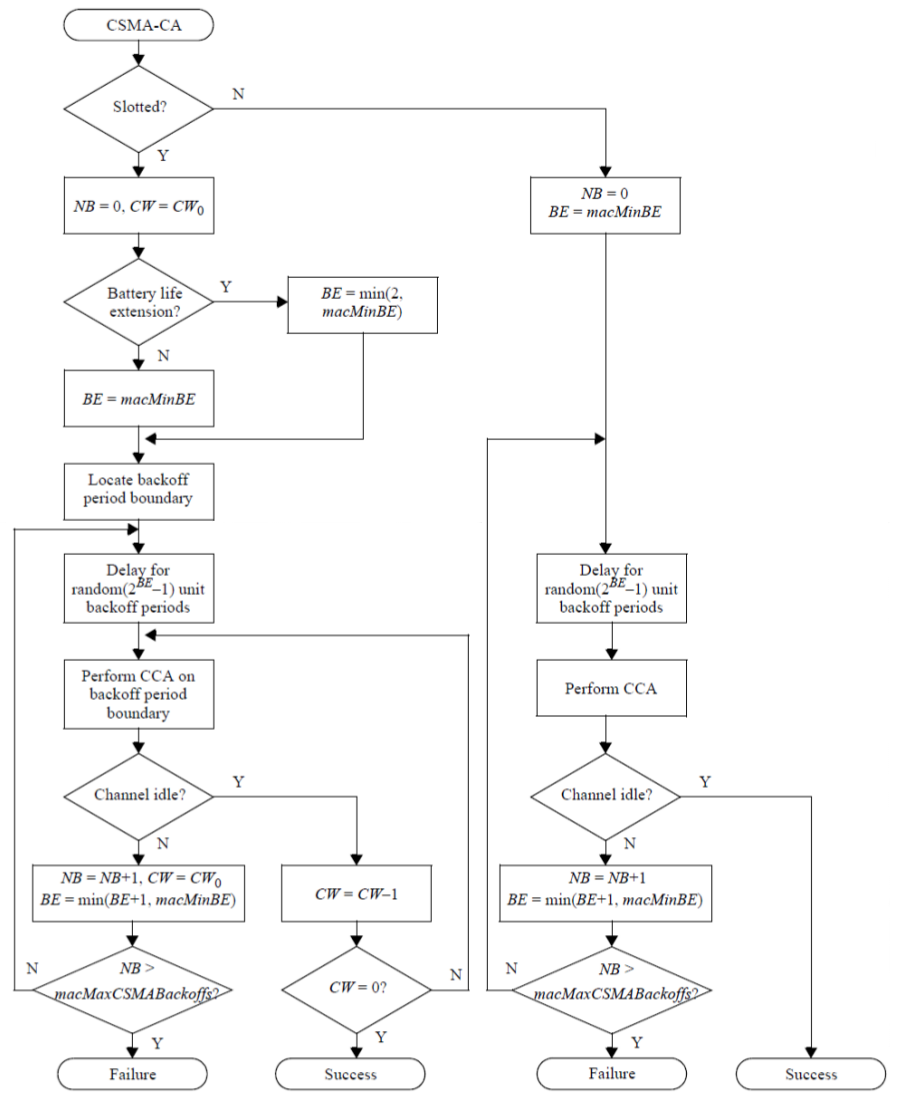
\includegraphics[width=14.25cm]{images/ch3-csma-ca-std.png}
\flcaption{Organigramme de l'algorithme de la m\'ethode CSMA/CA.
(Source~: \cite{IEEE802154-2011}, figure 11)}
\label{FigOrganigrammeCSMACA}
\end{figure}

En sus de la méthode CSMA/CA, notons qu'il existe également un mécanisme
obligatoire d'acquittement des trames. Ainsi, à la réception de chaque
trame de données, le noeud de destination doit renvoyer un acquittement
à l'envoyeur~; si après envoi d'une trame de données, le noeud émetteur
ne reçoit pas d'acquittement dans un délai voulu (\lang{``timeout''}),
l'envoi de la trame est considéré comme un échec.

\subsubsection{Mode \lang{``non-beacon''}}
\label{Par802154MACSimple}

Le mode de fonctionnement le plus simple de la couche MAC du standard
802.15.4 repose exclusivement sur l'emploi de la méthode CSMA/CA <<~non
slottée~>> décrite section \vref{ParCSMACA}. Il n'y a aucune notion de cycle
de fonctionnement~: le coordinateur est constammant en fonctionnement
(la plupart du temps en écoute), tandis que les noeuds simples n'accèdent
au médium radio que lorsqu'ils ont besoin d'envoyer ou recevoir des données.

La réception de données s'effectue grâce à un bit nommé \lang{``Frame
Pending''} de l'entête MAC 802.15.4, via lequel le coordinateur indique
à un de ses noeuds-feuilles qu'il attend de lui envoyer une trame lui
étant destinée. Le noeud destinataire peut alors envoyer une trame
spéciale dite <<~de commande~>> (\lang{``Data Request''}) pour déclencher
la réception proprement dite.

Ce mode est bien adapté aux réseaux dans lesquels les noeuds simples
émettent des données de façon sporadique (c'est-à-dire passent la
quasi-totalité de leur temps en <<~sommeil~>>), et où les données transmises
n'ont pas un caractère urgent (ce mode sans \lang{``beacon''} n'offrant
aucune garantie d'accès au canal pour une période donnée).

Il est ainsi possible d'avoir des noeuds simples fonctionnant sur une
batterie dont l'autonomie pourra être longue. Par contre, le noeud central
jouant le rôle de coordinateur doit lui être constamment à l'écoute, ce qui
impose la contrainte de le faire fonctionner sur une source d'énergie
constante (secteur).

\subsubsection{Mode \lang{``beacon''} (ou mode balisé)}
\label{Par802154MACBeacon}

Le second mode de fonctionnement de la couche MAC standard impose au
noeud central, jouant le rôle de coordinateur de PAN (compatible avec
celui de routeur, ce qui représente l'immense majorité des cas), l'envoi
régulier de \lang{``beacons''} à chaque début de cycle de fonctionnement
(\lang{``duty cycle''}).

Ces \lang{``beacons''} servent à synchroniser les différents noeuds du PAN
(ainsi qu'à identifier ce dernier).

Dans ce mode, un cycle de la couche se décompose en~:
\begin{description}
\item[l'envoi d'un \lang{``beacon''}] par le noeud coordinateur du PAN, cet
envoi n'utilisant pas la méthode CSMA/CA, mais la diffusion directe à tous
les noeuds à l'écoute (\lang{``broadcast''}), aucun autre noeud n'étant
en effet censé être autorisé à émettre spontanément hors cycle~;
le \lang{``beacon''} est, dans ce mode, en général la trame comportant
le fameux bit \lang{``Frame Pending''} pour permettre l'envoi de
données aux noeuds-feuilles~;
\item[une CAP] (\lang{Contention Access Period}) période durant laquelle
les noeuds simples émettent vers le noeud central, ou recoivent les données
leur étant destinées depuis celui-ci, en mode CSMA/CA~;
\item[une CFP] (\lang{Contention Free Period}) période durant laquelle
il est possible de garantir l'accès au médium radio pour un noeud (ou
plusieurs noeuds consécutifs)~;
\item[une période de sommeil] durant laquelle le PAN est mis en inactivité
ce qui permet aux différents noeuds, y compris le noeud central, de
désactiver leur émetteur~/ récepteur radio pour économiser leur énergie.
\end{description}

L'ensemble constitué par la CAP et la CFP d'un cycle donné constitue
la \nom{supertrame} (en anglais \lang{``superframe''}, par opposition
à la periode de sommeil).

Le cycle de fonctionnement du protocole MAC standard 802.15.4 en mode
\lang{``beacon''} est représenté dans la figure
\vref{FigMAC802154beacon}.

\begin{figure}[!hbt]
\centering
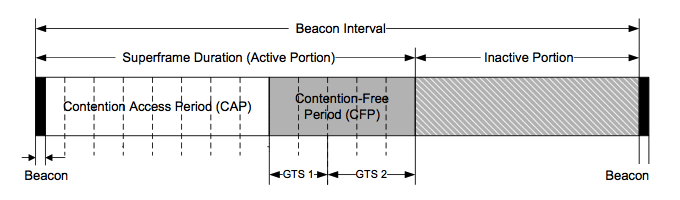
\includegraphics[width=12.5cm]{images/ch3-ieee802154-mode-beacon.png}
\flcaption{Cycle de fonctionnement du protocole MAC du standard IEEE
802.15.4 en mode \lang{``beacon''}.
(Source~: \cite{Evolution-MAC-WSN-Survey-2013})}
\label{FigMAC802154beacon}
\end{figure}

Cette supertrame est divisée en 16 \lang{``time slots''}, lequels sont
répartis entre CAP et CFP par le noeud coordinateur à chaque nouveau cycle,
en fonction des besoins du trafic réseau. Les \lang{``time slots''} alloués
à la CFP sont nommés \nom{GTS} (\lang{Guaranteed Time Slots})~; le standard
définit la procédure permettant à un noeud simple de demander au noeud
coordinateur de PAN de lui allouer un ou plusieurs GTS au cycle suivant.

On voit ainsi que ce mode offre plusieurs avantages par rapport au mode
\lang{``non-beacon''}~:
\begin{itemize}
\item le noeud coordinateur peut établir à lui seul son réseau (PAN)~;
\item la présence d'une CFP permet de prévoir l'envoi de données
importantes, dont le transport nécessite un accès garanti au médium
radio sans risque de collision~;
\item la CFP permet également d'envisager l'envoi de lots de trames
successifs (pour la transmission de données de grande taille), de façon
plus robuste que par l'utilisation de la méthode CSMA/CA.
\end{itemize}

On voit que la division de la période d'activité (\lang{superframe}) en CAP
et CFP est un moyen d'adapter le fonctionnement de la couche MAC au trafic
sur le médium radio. Par défaut, cette adaptabilité est limitée par le fait
que la durée d'un cycle, de la \lang{superframe}, et donc le rapport entre
ces deux durées, sont des constantes fixées lors de la configuration du PAN.
Des travaux ont récemment été menés pour adapter dynamiquement ces
paramètres au trafic réseau \cite{TheseSKhssibi}, le standard ne le
prévoyant pas, mais ne l'interdisant pas non plus.

\subsubsection{802.15.4e}
\label{Par802154e}

Le standard IEEE 802.15.4 continue à évoluer, et les groupes de travail
dédiés de l'IEEE ne cessent de le réviser et de le compléter~--- via
des amendements~--- au cours du temps.

Les amendements 802.15.4a, 4b, 4c et 4d ont successivement amené de
nouvelles bandes de fréquences et méthodes d'encodage du signal radio,
l'amendement IEEE 802.15.4a ayant notamment amené la notion d'UWB,
comme dit plus haut en section \vref{Subsec802154PHY}

Un amendement récent au standard, l'amendement 802.15.4e, adopté en 2012,
a ajouté une nouvelle couche MAC nettement plus complexe, incluant
notamment des mécanismes de multiplexage temporel \emph{et} fréquentiel
des transmissions radio. Nous reviendrons sur cet amendement 802.15.4e
dans la section \vref{SubsecProtoMACFDMA} consacrée aux protocoles MAC
multicanaux.


%%%%%%%%%%%%%%%%%%%%%%%%%%%%%%%%%%%%%%%%%%%%%%%%%%%%%%%%%%%%%%%%%%%%%%%%%%%%%

\section{Protocoles MAC}
\label{SecProtoMAC}

Outre les couches MAC <<~officielles~>> proposées par le standard
802.15.4, la communauté scientifique a proposé de nombreux protocoles
alternatifs destinés à surpasser les limitations du
protocole standard, notamment sa version simple reposant sur la seule
méthode CSMA/CA.

Contrairement au mode simple, et de façon similaire au mode balisé décrit
section \vref{Par802154MACBeacon}, ces protocoles MAC alternatifs
reposent sur la notion de \lang{``duty cycle''}. Toute la difficulté pour
la mise au point de ces protocoles consiste donc à fixer des \emph{points
de rendez-vous} entre les différentes noeuds pour assurer correctement
leur synchronisation.

On peut ainsi diviser ces divers protocoles en différentes familles, selon
les méthodes utilisées pour fixer ces points de rendez-vous~:

\begin{itemize}

\item les protocoles MAC synchrones, employant des mécanismes de
synchronisation explicites entre noeuds pour la transmission de trames~:
S-MAC et T-MAC en sont deux exemples~;

\item les protocoles MAC asynchrones basés sur l'écoute à basse énergie
(LPL~: \lang{Low Power Listening})~: B-MAC, X-MAC et ContikiMAC en sont
trois exemples (ce dernier étant aujourd'hui très largement utilisé)~;

\item les protocoles MAC asynchrones basés sur l'émission à basse énergie
(LPP~: \lang{Low Power Probing})~: RI-MAC en étant l'exemple le plus connu~;

\item les protocoles MAC basés sur l'ordonnancement temporel~: LMAC,
AI-LMAC en sont deux exemples~;

\item les protocoles MAC multicanaux~: différents protocoles ont exploré
cette voie, mais surtout, l'extension du standard IEEE 802.15.4e fait
désormais appel au multiplexage fréquentiel des transmissions, via un
mécanisme nommé TCSH.

\end{itemize}

Nous allons dans cette section étudier ces différents types de protocoles
de façon consécutive, à chaque fois en se penchant sur un ou deux
protocoles représentatifs de chaque famille (notre but n'étant ici
encore pas d'être exhaustif).

Enfin, nous étudierons plus en détail plusieurs protocoles MAC avancés~:
la famille CoSenS et iQueue-MAC, conçus et développés au sein du LORIA
et de l'INRIA Nancy, sur lequels nous avons focalisé nos travaux.

La présente section \ref{SecProtoMAC} reprend la présentation effectuée dans
les supports de cours de Y.-Q. Song sur les systèmes communicants contraints
\cite{coursEnsem}, ainsi que des données présentées dans l'article de
référence (\lang{``survey''}) de P. Huang, L. Xiao et al
\cite{Evolution-MAC-WSN-Survey-2013} et la thèse de B. Nefzi
\cite{TheseBNefzi}.


\subsection{Protocoles MAC synchrones}
\label{SubsecProtoMACSynchrones}

Cette famille de protocoles MAC est basée sur la synchronisation explicite
des cycles de fonctionnement de noeuds voisins. Il s'agit de la solution
la plus évidente pour permettre la communication entre appareils, mais
cela implique des coûts supplémentaires (en temps et en complexité)
pour effectuer cette synchronisation. Ce type de protocoles n'ayant
pas de difficultés pour établir des communications entre noeuds,
ils peuvent faire l'objet d'optimisations pour augmenter le débit
de données et réduire les délais de transmission.

\subsubsection{S-MAC}
\label{ParSMAC}

Un premier exemple de protocole synchrone est le protocole S-MAC \cite{SMAC}.
Celui-ci est basé sur la méthode CSMA/CA complétée par l'envoi de signaux
indiquant qu'un noeud a des données à envoyer (RTS~: \lang{Ready To Send})
et qu'un noeud est prêt à recevoir (CTS~: \lang{Clear To Send}). Ce mode
de fonctionnement est celui utilisé par le standard 802.11 (``Wi-Fi'').

Un cycle de fonctionnement sous le protocole S-MAC est divisé en une
période active et une période inactive. La période active est la seule
pendant laquelle un noeud peut envoyer et recevoir des données, la période
inactive correspondant à la désactivation de l'émetteur~/ récepteur radio
pour économiser l'énergie. La période active est elle-même divisée en
une période de synchronisation, et une période d'échange de données.

Dans ce protocole, chaque noeud choisit ses périodes actives et inactives
en fonction de ses voisins. Le premier noeud à démarrer est le seul
choisissant librement ses périodes, et annonce ensuite régulièrement
ses périodes par l'envoi de signaux de synchronisation (SYNC) durant
une période dédiée (au début de la période active). Les noeuds démarrant
ensuite vont alors adapter leurs propres périodes sur celles annoncées
par les noeuds précédents. Ce mécanisme d'adaptation porte le nom
\lang{``d'adaptative listening''}.

\begin{figure}[!hbt]
\centering
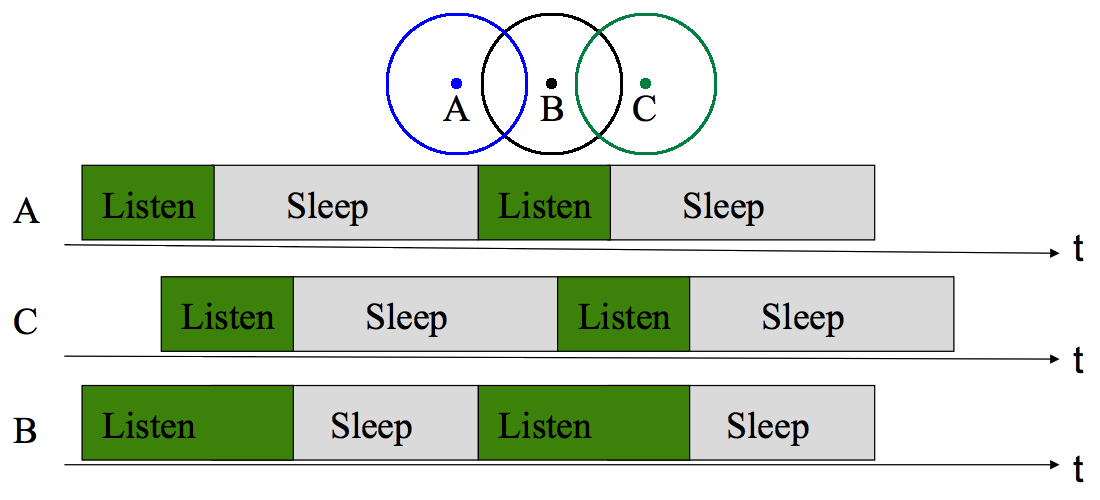
\includegraphics[width=12.5cm]{images/ch3-s-mac.png}
\flcaption{\lang{Adaptative listening} entre trois noeuds suivant
le protocole S-MAC.
(Source~: \cite{coursEnsem})}
\label{FigSMACadapt}
\end{figure}

La figure \vref{FigSMACadapt} montre un exemple de synchronisation
entre plusieurs noeuds sous S-MAC. Le noeud B, démarrant en dernier, adapte
sa période active à celle de ses deux voisins A et C. A et C étant hors de
portée l'un de l'autre, ne vont par contre pas se synchroniser entre eux.

Ce protocole est donc basé sur la définition de rendez-vous entre
émetteur et récepteur. L'utilisation de nombreux signaux pour coordonner
les transmissions (SYNC, RTS, CTS) entraîne un surcoût (\lang{``overhead''})
élevé diminuant d'autant la bande passante disponible pour les données,
même si S-MAC est capable d'envoyer des trames par lots (\lang{``send
burst''}), après une seule séquence RTS/CTS, pour accélérer le traitement
de données volumineuses.

Ce protocole ayant des cycles de fonctionnement fixes et un mécanisme
de synchronisation assez lourd, son adaptabilité au trafic sur le réseau
est très faible.

Notons enfin que toute synchronisation entre appareils différents est
susceptible d'être victime du phénomène de dérive des horloges (dû aux
inévitables différences de fonctionnement entre les horloges internes
de chaque appareil). S-MAC utilisant des périodes actives assez longues,
il est peu sensible aux perturbations dues à ce phénomène. 

\subsubsection{T-MAC}
\label{ParTMAC}

Le protocole T-MAC \cite{TMAC} est une amélioration de S-MAC. Dans T-MAC,
la durée de la période active n'est plus fixée à l'avance, mais chaque
noeud reste éveillé jusqu'à ce qu'aucun signal ne le concernant n'ait
été entendu pendant un certain délai (notion de \lang{``timeout''}).
Ce schéma permet un meilleure adaptabilité au trafic réseau, en permettant
notamment une période de sommeil plus longue en cas de faible trafic,
d'où une meilleure économie d'énergie. La figure \vref{FigSMACvsTMAC}
permet de comparer le fonctionnement de base des protocoles S-MAC et T-MAC.
On notera que ce dernier adapte sa période d'éveil à l'intensité du trafic
réseau.

\begin{figure}[!hbt]
\centering
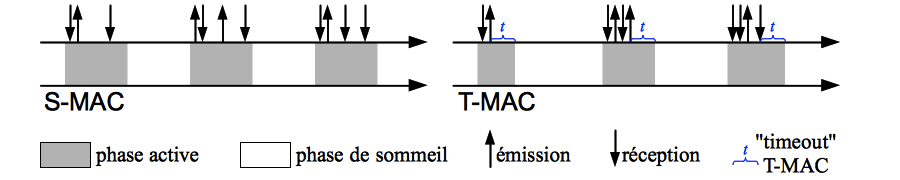
\includegraphics[width=12.5cm]{images/ch3-s-mac-vs-t-mac.png}
\flcaption{Comparaison du fonctionnement de S-MAC et T-MAC.
(Source~: \cite{coursEnsem})}
\label{FigSMACvsTMAC}
\end{figure}

T-MAC reprend également la capacité de S-MAC à effectuer des envois
de trames par lots (après une unique paire de signaux RTS/CTS) pour
un traitement plus efficace des données volumineuses.


\subsection{Protocoles MAC asynchrones LPL}
\label{SubsecProtoMACLPL}

Dans un protocole MAC asynchrone, chaque noeud garde sa propre base de temps
autonome. L'absence de synchronisation entre noeuds voisins permet (en
théorie) d'éviter d'employer des phases de synchronisation systématiques à
chaque cycle, donc à chaque appareil d'avoir un \lang{``duty cycle''} plus
réduit, et ainsi d'économiser son énergie, mais rend plus délicat
l'établissement de communications entre noeuds. Toute la difficulté
dans la mise au point d'un protocole asynchrone est de trouver une méthode
efficace en ce sens.

La famille des protocoles dits LPL (\lang{``Low Power Listening''}, ou
écoute à faible puissance) repose sur le principe suivant~: chaque noeud
passe la quasi-totalité de son temps en sommeil, c'est-à-dire avec sa radio
désactivée~; pour déterminer si un message lui est destiné, il va de façon
cyclique activer sa radio et vérifier si le canal radio est occupé
(la procédure consistant à écouter le médium radio pour vérifier s'il est
libre est appelée CCA~: \lang{Clear Channel Assessment}).

Les protocoles LPL vont différer sur la méthode d'envoi des données par les
noeuds émetteurs~: il s'agit en effet de s'assurer que le noeud destinataire
remarquera qu'une transmission lui est destinée~--- et donc d'entrer en
contact avec ce dernier lorsqu'il effectue son CCA~--- tout en essayant
de minimiser l'énergie consommée par le noeud émetteur (en limitant le
temps où la radio de ce dernier doit émettre).

\subsubsection{B-MAC}
\label{ParBMAC}

Un premier exemple de protocole LPL est B-MAC (Berkeley MAC) \cite{BMAC}.
Dans ce protocole, un noeud devant envoyer des données émet un très long
préambule (une trame ne contenant aucune donnée utile et ne servant qu'à
signaler une future émission de données). Ce préambule est très long car
son émission doit durer plus longtemps que l'intervalle entre deux CCAs
consécutifs du récepteur. De plus, ce préambule ayant une taille fixe,
le récepteur devra, lorsqu'il l'aura détecté, attendre sa fin avant de
pouvoir recevoir ses données proprement dites. Ce mode de fonctionnement
est représenté dans la figure \vref{FigBMAC}.

\begin{figure}[!hbt]
\centering
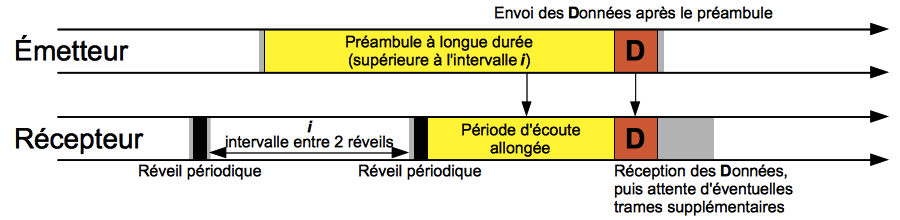
\includegraphics[width=12.5cm]{images/ch3-b-mac.png}
\flcaption{Schéma de fonctionnement de B-MAC (protocole LPL typique).
(Source~: \cite{coursEnsem})}
\label{FigBMAC}
\end{figure}

On voit que cette procédure entraîne une dépense d'énergie maximale pour
le noeud émetteur (à cause de la nécessité d'envoyer ce très long préambule)
ainsi qu'un encombrement important du canal radio, augmentant le risque
de collisions. La taille fixe du préambule comme de l'intervalle entre CCAs
consécutifs rend également le protocole très peu adaptable au trafic réseau.

\subsubsection{WiseMAC}
\label{ParWiseMAC}

Notre second exemple de protocole LPL, nommé WiseMAC \cite{WiseMAC},
emploie une technique consistant à <<~apprendre~>> les cycles de
fonctionnement des noeuds voisins d'un même PAN. Pour ce faire, ce
protocole repose d'abord sur l'envoi de longs préambules (comme B-MAC),
auquels les noeuds récepteurs du PAN répondent par un acquittement lors
de leur phase cyclique de réveil (\lang{``channel sampling''}).
Une fois les cycles de tous les noeuds du PAN connus, WiseMAC se distingue
alors de B-MAC, en recourant à l'envoi de préambules bien plus courts,
ce qui est possible en démarrant les transmissions au moment adéquat
(en incluant une certaine marge de sécurité pour éviter les problèmes
dûs à la dérive des horloges entre appareils). La possibilité, après
un temps d'apprentissage, d'utiliser des préambules raccourcis améliore
considérablement la consommation d'énergie des différents noeuds~---
aussi bien des émetteurs ayant moins de temps à passer à émettre, que
des récepteurs n'ayant plus à écouter inutilement des préambules trop
longs~--- et optimise l'utilisation du médium radio en le libérant
pour la transmission de données <<~utiles~>>, augmentant ainsi le
débit maximal utile réel du réseau.

\subsubsection{X-MAC}
\label{ParXMAC}

Notre troisième exemple de protocole LPL, X-MAC \cite{XMAC}, optimise
nettement la procédure d'envoi, en remplaçant les long préambules de B-MAC
par de très courts trames-préambules intégrant en outre l'adresse du
noeud destinataire, comme on peut le voir dans la figure \vref{FigXMAC}.
Cette technique améliore non seulement la dépense d'énergie par le noeud
émetteur ainsi que le taux d'occupation du médium, mais permet également
d'éviter de garder inutilement éveillés des noeuds tiers, le destinataire
d'une future émission étant clairement identifié par ces courts préambules.
Enfin, X-MAC inclut également l'envoi d'un acquittement préalable par le
noeud récepteur (assimilable à un signal CTS) avant l'envoi des données
proprement dites. 

\begin{figure}[!hbt]
\centering
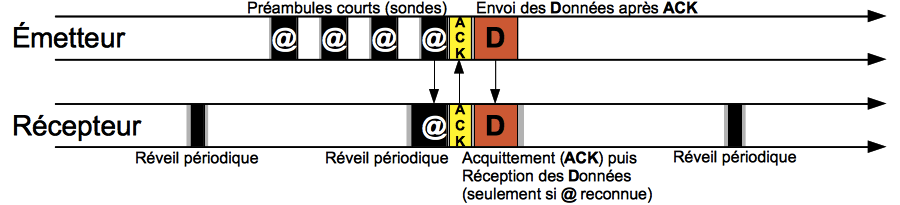
\includegraphics[width=12.5cm]{images/ch3-x-mac.png}
\flcaption{Schéma de fonctionnement du protocole X-MAC.
(Source~: \cite{coursEnsem})}
\label{FigXMAC}
\end{figure}

\subsubsection{ContikiMAC}
\label{ParContikiMAC}

Notre quatrième exemple de protocole LPL est ContikiMAC \cite{ContikiMAC}.
Celui-ci est nettement plus récent que les précédents, et a été conçu
spécifiquement pour fonctionner sous Contiki OS (système que nous
présenterons dans la section \vref{SubsecContikiOS}).

Ce protocole, par rapport à X-MAC, simplifie encore la procédure d'envoi
des données, en supprimant totalement la notion de préambule~: lors d'une
transmission, c'est désormais la trame de données elle-même qui est
émise de façon répétitive, jusqu'au prochain réveil du noeud récepteur.
Une fois la trame de données bien reçue, le destinataire envoie un
acquittement (ACK standard 802.15.4) pour mettre fin à l'émission de la
trame. Le fonctionnement de ContikiMAC est représenté
dans la figure \vref{FigContikiMAC}.

\begin{figure}[!hbt]
\centering
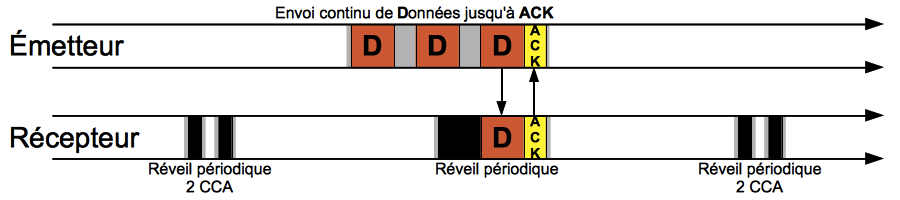
\includegraphics[width=12.5cm]{images/ch3-contikimac.png}
\flcaption{Schéma de fonctionnement du protocole ContikiMAC.
(Source~: \cite{coursEnsem})}
\label{FigContikiMAC}
\end{figure}

Autre particularité~: chaque noeud effectue \emph{deux} CCA à chaque réveil
cyclique, et ne retombe en sommeil que si ces deux CCA ont indiqué
la non-occupation du canal radio. (Ces deux CCA, séparés par un délai
calculé à partir du délai standard entre émission de trames (DIFS)
et la taille minimale d'une trame 802.15.4, permettent de consommer
moins d'énergie qu'une longue écoute. Ces deux CCA ont ainsi la durée
minimale nécessaire pour déterminer ou non l'occupation du médium radio.)

Enfin, signalons que les versions récentes de ContikiMAC bénéficient d'une
optimisation supplémentaire~: après un envoi réussi, le noeud émetteur
mémorise la période de réveil du destinataire, afin d'envoyer les
trames suivants au meilleur moment et ainsi limiter au maximum
les transmissions inutiles. Cette optimisation est nommée \lang{``phase
lock''} par les concepteurs de ContikiMAC. \\
On peut rapprocher cette technique de \lang{``phase lock''} du mécanisme
d'apprentissage des cycles des noeuds observé antérieurement dans le
protocole WiseMAC.


\subsection{Protocoles MAC asynchrones LPP}
\label{SubsecProtoMACLPP}

Si les protocoles LPL sont conçus pour avoir une meilleure adaptabilité
au trafic que les protocoles synchrones (comme S-MAC ou T-MAC),
ils souffrent néanmoins de plusieurs inconvénients~:
\begin{itemize}
\item une efficacité energétique non optimale~: B-MAC, avec ses très longs
préambules, est clairement insuffisant dans ce domaine~;
\item l'envoi de préambules (ou de trames dans le cas de ContikiMAC)
avant la <<~transmission réelle~>> occupe inutilement le medium,
augmentant ainsi les délais de transmission, les risques de collision,
et diminuant le débit réel maximal du trafic~;
\item l'inadéquation aux trafics élevés~--- par exemple lors de <<~pics~>>
ou <<~pointes~>> de transmissions~--- à cause de la méthode CSMA/CA
sous-jacente~;
\item la risque de <<~collisions cachées~>> entre noeuds~: ce terme
regroupe les cas où plusieurs paires de noeuds émetteurs/récepteurs,
ayant chacune indépendemment des données à se transmettre, se gênent
mutuellement si elles sont partiellement à portée l'une de l'autre.
La figure \vref{FigCollisionsCachees} illustre la survenue
d'un de ces problèmes~: les deux récepteurs sont à portée des deux
émetteurs, ces derniers étant par contre incapables de se détecter
mutuellement, ce qui provoque une collision entre les trames transmises
par chacun des deux émetteurs.
\end{itemize}

\begin{figure}[!hbt]
\centering
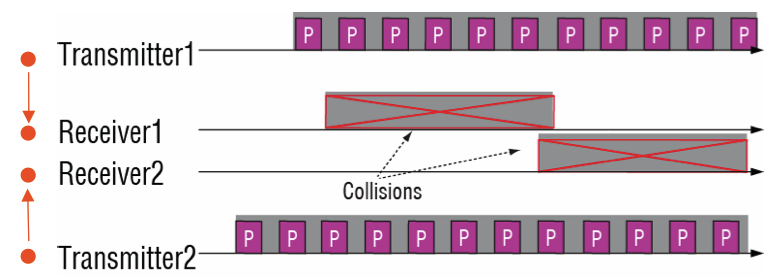
\includegraphics[width=12.5cm]{images/ch3-collisions-cachees.png}
\flcaption{Survenue d'une <<~collision cachée~>> entre deux paires
de noeuds menant chacun une transmission distincte, empêchant
la réussite des deux communications.
(Source~: \cite{coursEnsem} d'après \cite{RIMAC})}
\label{FigCollisionsCachees}
\end{figure}

Pour tenter de résoudre ces problèmes, un autre famille de protocoles
MAC asynchrones a été conçue. Elle repose sur l'idée fondamentale
de laisser les noeuds destinataires démarrer les transmissions.
On parle donc de communications initiées par le recepteur, chaque noeud
émettant cycliquement des \lang{``beacons''} (ou \lang{``probes''}~: sondes)
signalant quand il est prêt à recevoir (RI-LPP~: \lang{Receiver Initiated
Low Power Probing}).

\subsubsection{RI-MAC}
\label{ParRIMAC}

L'exemple de protocole LPP que nous allons examiner ici est RI-MAC
\cite{RIMAC}. Son principe de fonctionnement est le suivant~: chaque
noeud d'un réseau se réveille périodiquement, et émet un \lang{``beacon''}
signalant qu'il est prêt à recevoir des données. Un noeud ayant des données
à transmettre va donc écouter le médium radio et attendre de recevoir
un \lang{``beacon''} issu du destinataire voulu. Dès ce \lang{``beacon''}
reçu, l'émetteur envoie sa trame de données. Le noeud récepteur confirmera
ensuite la bonne réception de cette trame par l'envoi d'un nouveau
\lang{``beacon''}, lequel joue à la fois le rôle d'acquittement de la trame
reçue (ACK) \emph{et} de signal pour le lancement d'une nouvelle transmission.
Grâce à ce double rôle des \lang{``beacons''}, l'envoi rapide de trames
par lots est possible (par exemple pour gérer les transmissions de grandes
quantités de données). Le principe de fonctionnement de la méthode LPP
est représentée dans la figure \vref{FigPrincipeLPP}.

\begin{figure}[!hbt]
\centering
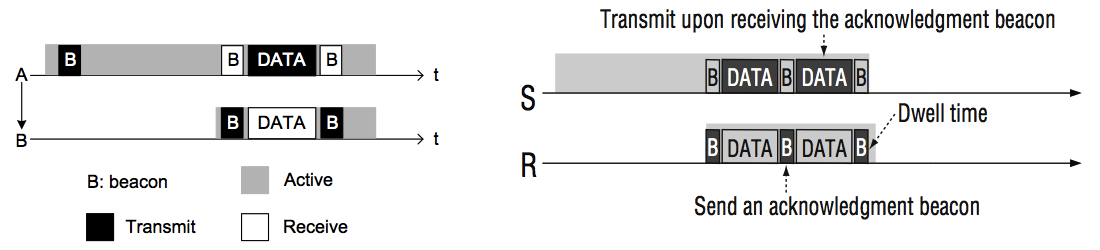
\includegraphics[width=14cm]{images/ch3-lpp.png}
\flcaption{Principe de transmission de données entre un noeud émetteur
(\textbf{A} ou \textbf{S}) et un noeud récepteur (\textbf{B} ou
\textbf{R}), selon la méthode RI-LPP (\lang{Receiver-Initiated
Low Power Probing}).
(Source~: \cite{coursEnsem} et \cite{Evolution-MAC-WSN-Survey-2013})}
\label{FigPrincipeLPP}
\end{figure}

Par rapport aux protocoles LPL, ce principe de fonctionnement permet
de réduire l'occupation moyenne du médium radio par un couple de
noeuds pour arriver à un point de rendez-vous.
En outre, les phénomènes de collisions cachées entre noeuds sont
également moins fréquents.

L'un des principaux problèmes du principe LPP survient lorsque
plusieurs noeuds ont simultanément besoin d'envoyer des données
au même destinataire~: à la réception du \lang{``beacon''} émis par ce
dernier, les différents noeuds émetteurs vont tous émettre leurs
trames de données, ce qui provoquera inévitablement une collision.
La probabilité que plusieurs noeuds cherchent à envoyer des données
au même noeud au même moment est d'autant plus forte que le trafic
du réseau concerné devient important.

Pour pallier ce problème, RI-MAC ajoute au principe LPP de base
une notion de \lang{``backoff''} intégrée aux \lang{``beacons''}~:
ces derniers incluent en effet une durée maximale de <<~silence~>>
parmi laquelle les noeuds émetteurs devront choisir aléatoirement
un délai à respecter entre la réception de ce \lang{``beacon''} et
l'envoi de leurs données. Au début, cette fenêtre de \lang{``backoff''}
est nulle~; à chaque collision détectée, cette fenêtre va voir
sa valeur augmenter rapidement pour minimiser les risques de nouvelle
collision. Cette procédure est appelée BEB (\lang{Binary Exponential
Backoff}), et est illustrée dans la figure \vref{FigBEBRIMAC}.

\begin{figure}[!hbt]
\centering
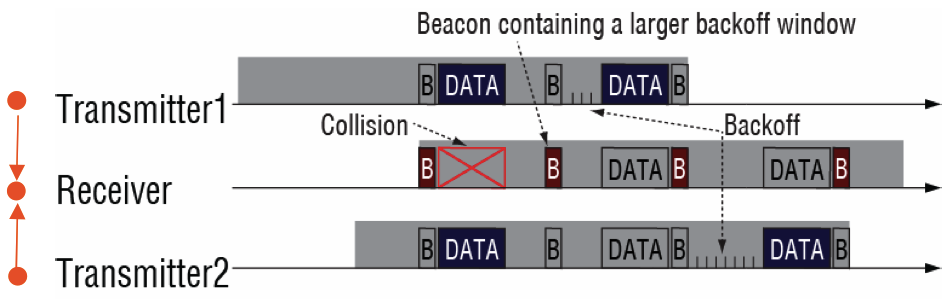
\includegraphics[width=12.5cm]{images/ch3-ri-mac-backoff.png}
\flcaption{Illustration de la méthode BEB (\lang{Binary Exponential
Backoff}) employée par RI-MAC pour résoudre les problèmes de
collisions dûs à l'envoi simultané de trames par plusieurs
émetteurs.
(Source~: \cite{coursEnsem} d'après \cite{RIMAC})}
\label{FigBEBRIMAC}
\end{figure}

On peut noter que cette procédure de BEB est similaire au mécanisme de
\lang{``backoff''} utilisé par la méthode CSMA/CA, également dans le but
de résoudre les cas de collisions.

\medskip

Grâce à ces mécanismes de fonctionnement, RI-MAC peut obtenir de meilleurs
résultats que X-MAC quand le trafic réseau est élevé, tout en ayant
un cycle de fonctionnement similairement bas (donc aussi économe en
énergie) quand le trafic est faible.

De façon générale, on constate que les protocoles basés sur le principe
RI (\lang{Receiver Initiated}) sont nettement plus performants quand le
trafic réseau est intense et/ou soumis à des interférences, là où les
protocoles laissant l'initiative de la transmission aux émetteurs vont
<<~étouffer~>> le réseau avec des collisions de trames de données.
Cela est nettement visible dans le schéma présenté dans la figure
\vref{FigRIvsSI}. On y voit que les protocoles
\lang{``Receiver-Initiated''} (LPP) ont toujours un net avantage,
d'autant plus flagrant que le débit augmente.

\begin{figure}[!hbt]
\centering
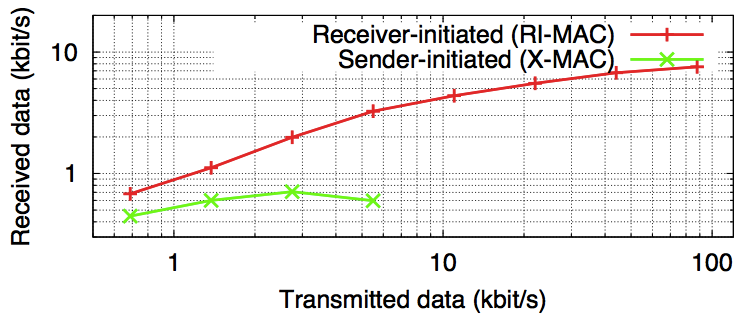
\includegraphics[width=12.5cm]{images/ch3-ri-vs-si.png}
\flcaption{Comparaison entre protocoles \lang{``Receiver-Initiated''} (LPP)
et \lang{``Sender-Initiated''} (LPL) face à la montée en charge
du trafic réseau.
(Source~: \cite{coursEnsem} d'après \cite{Strawman})}
\label{FigRIvsSI}
\end{figure}

Néanmoins, l'utilisation du médium radio par la méthode LPL (même améliorée
par RI-MAC) est toujours loin d'être optimale, le recours aux \lang{backoffs}
aléatoires pour éviter les collisions provoquant des <<~temps morts~>> où
le réseau doit rester inutilement silencieux.


\subsection{Protocoles MAC à ordonnancement temporel}
\label{SubsecProtoMACTDMA}

Tous les protocoles que nous avons vus jusqu'ici sont basés sur la
\emph{contention}~: les trames de données sont émises sur un médium radio
non réservé, ce qui implique un risque de collision et donc de perte de
données (ce qui nécessite en général un mécanisme de vérification et de
réémission des données si besoin est).

À l'inverse, les protocoles MAC dit \emph{ordonnancés} définissent
strictement l'occupation du médium radio, en allouant une partie
précise de la bande passante à chaque transmission potentielle, éliminant
ainsi les collisions.

La méthode employée pour parvenir à cette fin est basée sur le multiplexage
temporel~: chaque transmission se voit allouer le canal radio durant un
intervalle de temps bien défini. Cette méthode de fonctionnement est nommée
\nom{TDMA} (\lang{Time Division Multiple Access}). Son fonctionnement est
très similaire à la CFP observée plus haut dans le protocole MAC du standard
IEEE 802.15.4 en <<~mode \lang{``beacon''}~>>.

\begin{itemize}

\item Les protocoles basés sur la méthode TDMA sont considérés comme les
plus efficaces pour le traitement de trafics réseaux intenses, car ce sont
ceux qui permettent d'exploiter le plus efficacement le médium radio, et
donc d'approcher le plus de son débit maximal théorique.

\item Par contre, la nécessité de réserver au préalable les différents
intervalles de temps, quelle que soit l'intensité du trafic réseau, entraîne
un surcoût d'organisation (\lang{``overhead''}), ce qui rend les protocoles
basés sur la contention plus efficaces pour les faibles trafics. Les réseaux
de capteurs sans-fil actuels n'ayant le plus souvent à gérer qu'un faible
trafic (avec éventuellement quelques pointes), cela explique que les
protocoles basés sur la contention restent actuellement les plus utilisés.

\end{itemize}

Tout ceci est résumé de façon claire et synthétique dans le schéma présenté
dans la figure \vref{FigTDMAvsCSMA}. On y voit que la contention (CSMA)
gère mieux les faibles trafics, tandis que l'ordonnancement (TDMA) est plus
efficace pendant les débits intenses (ou les pointes de trafic réseau).

\begin{figure}[!hbt]
\centering
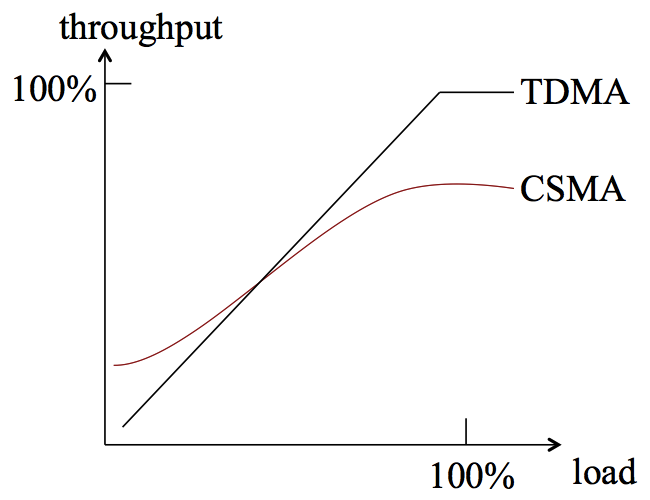
\includegraphics[width=10cm]{images/ch3-tdma-vs-csma.png}
\flcaption{Comparaison de l'efficacité entre méthodes basée sur la
contention (CSMA) et sur l'ordonnancement (TDMA) en fonction du débit
réseau.
(Source~: \cite{coursEnsem})}
\label{FigTDMAvsCSMA}
\end{figure}

En outre, toujours à cause de la nécessité d'organisation préalable
du multiplexage temporel du médium radio, les protocoles basés sur
l'ordonnancement sont en général du type synchrone, bien mieux adapté.

\subsubsection{LMAC}
\label{ParLMAC}

Le protocole LMAC \cite{LMAC} est un exemple typique de protocole basé
sur la méthode TDMA. Chaque cycle de fonctionnement (ou <<~trame~>>)
est divisé en \lang{``slots''}, représentant une unité minimale de temps
qui sera réservée à un noeud donné. Chaque noeud du réseau se verra
attribuer un \lang{slot} donné au sein de chaque trame réseau.

Durant son \lang{slot} de temps, un noeud doit d'abord émettre un
message de contrôle~--- indiquant s'il a des données à transmettre,
et si oui quel est leur destinataire~--- suivi s'il y a lieu du trame
de données à émettre.

Tous les noeuds du réseau doivent ainsi avoir leur émetteur~/ récepteur
radio activé pour écouter le message de contrôle émis au début de chaque
\lang{slot}. Les noeuds n'étant pas destinataires d'un message durant ce
\lang{slot} peuvent ensuite désactiver leur radio (donc tous les
noeuds si aucune donnée n'est à émettre durant ce \lang{slot}).

À noter que l'allocation des slots ne se fait pas de façon centralisée~:
au démarrage du réseau, chaque noeud doit choisir un \lang{slot} parmi
ceux disponibles, et le réserver pour les trames suivantes en y émettant
un message de contrôle.

\subsubsection{AI-LMAC}
\label{ParAILMAC}

Le protocole AI-LMAC \cite{AILMAC} est une extension de LMAC permettant
à un noeud de réserver plusieurs \lang{slots} au sein de chaque trame.
Le choix du nombre de \lang{slots} à allouer à chaque noeud n'est pas
faite de façon distribuée (comme pour la réservation), mais par le
coordinateur du réseau en fonction du trafic sortant prévu pour
chaque noeud.


\subsection{Protocoles MAC multicanaux}
\label{SubsecProtoMACFDMA}

Une dernière catégorie de protocoles MAC repose sur la capacité de la
couche physique 802.15.4 d'exploiter plusieurs canaux (c'est-à-dire
plusieurs fréquences) radio différents. Ainsi, tout comme il est possible
de multiplexer les différentes transmissions dans le temps, cette
fonctionnalité de la couche physique permet d'effectuer un multiplexage sur
les fréquences radio~: en assignant des canaux différents aux différents
noeuds d'un réseau, il devient possible de gérer des transmissions de
données parallèles.

Par analogie avec l'acronyme TDMA vu section \vref{SubsecProtoMACTDMA},
cette méthode de multiplexage sur les fréquences radio est appelée
\nom{FDMA} (\lang{Frequency Division Multiple Access}).

Les deux principales difficultés pour la conception de tels protocoles sont~:
\begin{itemize}
\item la distribution des différents canaux aux différents noeuds
d'un réseau~; et
\item la gestion efficace de la communication entre ces différents canaux.
\end{itemize}
Le deuxième point est rendu particulièrement difficile, car les émetteurs~/
récepteurs radio conçus pour le standard 802.15.4 ne sont pas capables
d'écouter simultanément plusieurs fréquences.
En outre, le standard 802.15.4 limitant la taille des trames physiques
à 127 octets, un mécanisme d'attribution des canaux aux différents noeuds
peut rapidement entraîner un surcroît de charge (\lang{``overhead''})
intolérable pour un réseau de ce type.

Différents protocoles ont été proposés pour contourner ces difficultés,
la tendance actuelle étant de combiner multiplexage temporel et multiplexage
fréquentiel~: on parle ainsi de protocoles TDMA/FDMA. Parmi ces protocoles,
on peut citer MC-LMAC employant cette méthode pour gérer les envois de
reales de données, ainsi que Y-MAC et MuChMAC employant une méthode
de <<~saut de fréquence~>> (\lang{``channel hopping''}) pour permettre
aux différents noeuds de recevoir des trames de données de plusieurs
canaux différents.

Ces protocoles multicanaux n'ayant pas été traités lors des présents
travaux de thèse, nous ne les étudierons pas plus en détail ici~;
l'étude de référence (\lang{``survey''}) de
\cite{Evolution-MAC-WSN-Survey-2013} consacrant toute sa section V
à l'étude de ces protocoles, nous invitons le lecteur souhaitant plus
de détails sur ce sujet à s'y reporter.

Il est par contre plus important de noter que l'amendement \nom{802.15.4e}
du standard, adopté en 2012, consacré à l'amélioration de la couche MAC
officielle du standard IEEE \cite{IEEE802154e-2012}, inclut un mécanisme
nommé \lang{``Time Slotted Channel Hopping''} ou \nom{TSCH}. Plus qu'une
simple amélioration, il s'agit tout simplement d'une nouvelle couche MAC,
totalement compatible avec la couche physique définie dans les précédentes
versions du standard 802.15.4, employant multiplexage temporel \emph{et}
multiplexage fréquentiel pour parvenir à une consommation d'énergie
minimale et une fiabilité de transmission maximale.

Une version dédiée de la pile IPv6 destinée à fonctionner par-dessus cette
nouvelle couche MAC et son mécanisme TSCH est déjà en cours de conception
par l'IETF, sous le nom de projet <<~6TiSCH~>> \cite{6TiSCH}. Cette nouvelle
pile protocolaire est notamment destinée à être supportée par la pile
réseau avancée \nom{OpenWSN} \cite{OpenWSN}, dont nous reparlerons
dans plus loin dans le présent chapitre (section \vref{SubsecRIOTOS}
sur RIOT OS et section \vref{SubsecFreeRTOS} sur FreeRTOS).

Notons toutefois que cette couche MAC est largement plus complexe que celles
définies dans les versions précédentes du standard (et que nous avons
étudiées section \vref{Subsec802154MAC}). Sa mise en oeuvre pourrait
par conséquent poser des difficultés sur les appareils à fonctionnalités
réduites (RFD) susceptibles de faire partie d'un réseau de capteurs sans-fil.
La description de cette nouvelle couche MAC complexe sort du cadre du
présent manuscrit de thèse et ne sera donc pas entreprise ici.

Malgré ces limitations, le standard IEEE 802.15.4e proposant désormais une
couche MAC officielle reposant sur le paradigme TDMA/FDMA, ce mode de
fonctionnement sera sans doute appelé à devenir incontournable dans
l'implantation des réseaux de capteurs sans-fil du futur.

\bigskip

Après l'étude des principales catégories <<~standard~>> de protocoles MAC,
et d'exemples représentatifs de ces dernières, nous allons maintenant nous
focaliser sur les protocoles avancés ayant fait l'objet des travaux de
la présente thèse.


\subsection{Protocoles hybrides avancés}
\label{SubsecProtoMACavances}

Des recherches sur la conception de protocoles MAC ont également été menées
au sein du centre INRIA Nancy Grand-Est et du LORIA. Ces recherches ont
notamment abouti à la conception de plusieurs protocoles évolués, qui ont
été à la base des travaux menés dans la présente thèse. Nous allons dans
la présente section examiner successivement ces différents protocoles
sur lesquels nous nous sommes focalisés.

Nous aborderons également brièvement~--- pour compléter notre tour d'horizon
des protocoles avancés~--- dans une autre sous-section les travaux d'autres
équipes de recherche sur d'autres protocoles MAC avancés.

Nous évoquerons aussi la couche MAC contenue dans une pile protocolaire
intégrée et complète, issue d'un effort de développement suivant une approche
dite multi-couches (en anglais \lang{``cross-layer''} dans une dernière
sous-section. De telles approches sortent toutefois du cadre de cette thèse,
laquelle se focalise sur les seules couches basses, et ne font par conséquent
l'objet d'aucun travail dans cette thèse.

\subsubsection{CoSenS et S-CoSenS}
\label{ParSCoSenS}

Ce protocole, conçu par B. Nefzi et Y.-Q. Song \cite{CosensConf}
\cite{CosensJournal}, fait partie de la classe des protocoles basés sur
la contention. Il est décrit dans le chapitre 3 de la thèse
de B. Nefzi \cite{TheseBNefzi}.

Le but de ce protocole est d'améliorer les performances de la couche
MAC notamment concernant la qualité de service, tout en limitant les coûts
liés à l'implantation de cette couche, ce qui exclut le recours à la
méthode TDMA (celle-ci nécessitant une configuration minutieuse
du réseau, une précision très fine de la synchronisation entre noeuds,
et une adaptation difficile aux changements de trafic sur le réseau).

Le protocole CoSenS reprend donc la méthode CSMA/CA, en contrôlant
les instants où se déroulent les transmissions et où le médium radio
est utilisé. Le principe de base est de séparer temporellement la période
où un noeud reçoit des trames de données (période de réception) de celle
où ce même noeud émet les trames ainsi reçues (période de retransmission).
Ceci est schématisé dans la figure \vref{FigCoSenSBase}. On voit que
chaque cycle CoSenS est partagé entre une période de réception (ou période
d'écoute~: WP) durant laquelle le noeud collecte les trames reçues,
suivi d'une période de transmission (TP) durant laquelle tous les trames
collectées dans la file d'envoi sont transmises vers la destination
adéquate. (Les trames~/ paquets collectés pouvant éventuellement être
traités par les couches supérieures de la pile de façon arbitraire
entre réception et émission).

\begin{figure}[!hbt]
\centering
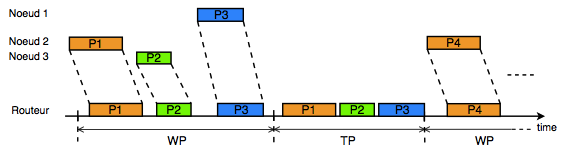
\includegraphics[width=12.5cm]{images/ch3-cosens-base.png}
\flcaption{Principe de base du protocole CoSenS.
(Source~: \cite{TheseBNefzi})}
\label{FigCoSenSBase}
\end{figure}

Il a été démontré que ce protocole apporte une amélioration sensible
des performances et de la qualité de service~--- notamment au niveau
du taux de succès de transmission des trames, du débit réseau maximal
supporté, ainsi que du délai de transmission de bout-en-bout des données~---
par rapport au protocole MAC de base du standard 802.15.4.

\newpage

Son principal défaut est par contre de nécessiter que tous les noeuds
gardent leur émetteur~/ récepteur radio allumé en permanence, ce qui
représente un sérieux désavantage concernant l'économie d'énergie.

C'est pourquoi ce protocole a été amélioré pour inclure une période
de sommeil dans le cycle de fonctionnement des noeuds. Le protocole
résultant est nommé \nom{S-CoSenS}, et c'est celui sur lequel nous
nous sommes principalement basés lors de nos travaux de thèse. Il s'agit
donc à la fois d'un protocole MAC et d'un protocole RDC (\lang{Radio
Duty Cycle}~: gérant le cycle d'allumage et d'extinction de l'émetteur~/
récepteur radio), qui plus est adapté aux phases de routage. Il est décrit
dans le chapitre 5 de la thèse de B. Nefzi \cite{TheseBNefzi}.

Tout comme CoSenS, il est basé sur la méthode CSMA/CA, et est ainsi
comparable à la couche MAC 802.15.4 en <<~mode sans \lang{``beacon''}~>>.
L'idée de base reste de retarder la retransmission des trames reçues,
en divisant chaque cycle de fonctionnement d'un noeud coordinateur
en trois périodes~:
\begin{itemize}
\item une période de sommeil (SP~: \lang{Sleeping Period}) où l'émetteur~/
récepteur radio est désactivé pour économiser l'énergie du noeud~;
\item une période d'écoute ou période d'attente (WP~: \lang{Waiting Period})
durant laquelle le médium radio est écouté pour collecter les trames de
données 802.15.4 arrivantes~;
\item et une période de transmission (TP~: \lang{Transmission Period})
durant laquelle les trames reçues et mis en attente durant la période
d'écoute sont réémises, si possible en lot (\lang{``burst''}).
\end{itemize}

Le principal avantage de S-CoSenS est son capacité à s'adapter dynamiquement
à l'intensité du trafic radio en temps réel, en calculant pour chaque cycle
radio (commun à tout un PAN fonctionnant sous S-CoSenS) la durée des
périodes de sommeil (SP) et d'écoute (WP), en fonction du nombre de
trames retransmises durant les cycles précédents.

Notons que l'ensemble constitué de la période de sommeil (SP) et de la
période de réception (WP) d'un même cycle est appelé \nom{subframe}~;
il s'agit de la partie du cycle de S-CoSenS dont la durée est calculée
et connue \lang{a priori}. À l'inverse, la durée de la période d'envoi (TP)
ne peut être déterminée qu'à son tout début, car cette durée dépend
directement de la quantité de trames de données reçues avec succès
durant la période d'écoute (WP) précédente.

En outre, le calcul de la durée de la période d'envoi WP se fait via un
algorithme de <<~moyenne glissante~>>, où la durée de WP pour chaque cycle
est calculée ainsi~:
\begin{eqnarray*}
&&
\overline{\mathrm{WP}_{n}} = \alpha \cdot \overline{\mathrm{WP}_{n-1}}
                + (1 - \alpha) \cdot \mathrm{WP}_{n-1}
\\ &&
\mathrm{WP}_{n} = \max ( \mathrm{WP}_{min},
                  \min ( \overline{\mathrm{WP}_{n}}, \mathrm{WP}_{max} ) )
\end{eqnarray*}
où $\overline{\mathrm{WP}_{n}}$ et $\overline{\mathrm{WP}_{n-1}}$
sont respectivement la durée moyenne de WP au $n^{\mathrm{eme}}$ et
$(n-1)^{\mathrm{eme}}$ cycle, tandis que $\mathrm{WP}_{n}$ et
$\mathrm{WP}_{n-1}$ sont les durées réelles de WP respectivement
au $n^{\mathrm{eme}}$ et $(n-1)^{\mathrm{eme}}$ cycles;
$\alpha$ est un paramètre dont la valeur est arbitrairement choisie
entre 0 et 1, représentant le poids relatif de l'historique dans le
calcul des durées~; $\mathrm{WP}_{min}$ et $\mathrm{WP}_{max}$ étant
les limites minimales et maximales imposées à la durée de WP par
le programmeur.

La synchronisation locale entre un routeur S-CoSenS et ses noeuds-feuilles,
au sein d'un même PAN, se fait grâce à une trame \lang{``beacon''}
émis par le routeur au début de chaque cycle. Ce \lang{``beacon''} inclut
les durées (en microsecondes) choisies pour la période de sommeil (SP) et
la période de réception (WP) au cours du cycle dont le \lang{``beacon''}
marque le début.

La représentation schématique d'un cycle complet S-CoSenS,
du point de vue d'un routeur gérant un PAN, est décrite dans la figure
\vref{FigCycleSCoSenS}. On distingue la période de sommeil (SP),
la période d'écoute~/ réception (WP) et la période de retransmission (TP).
L'ensemble des deux premières périodes constitue la \lang{subframe},
dont la durée est calculée à l'avance, en fonction du trafic
réseau observé jusqu'alors.

La figure \vref{FigCycleSCoSenS} montre clairement l'adaptation
du cycle S-CoSenS à un trafic réseau moyen (a), intense (b) et faible (c).

\begin{figure}[!hbt]
\centering
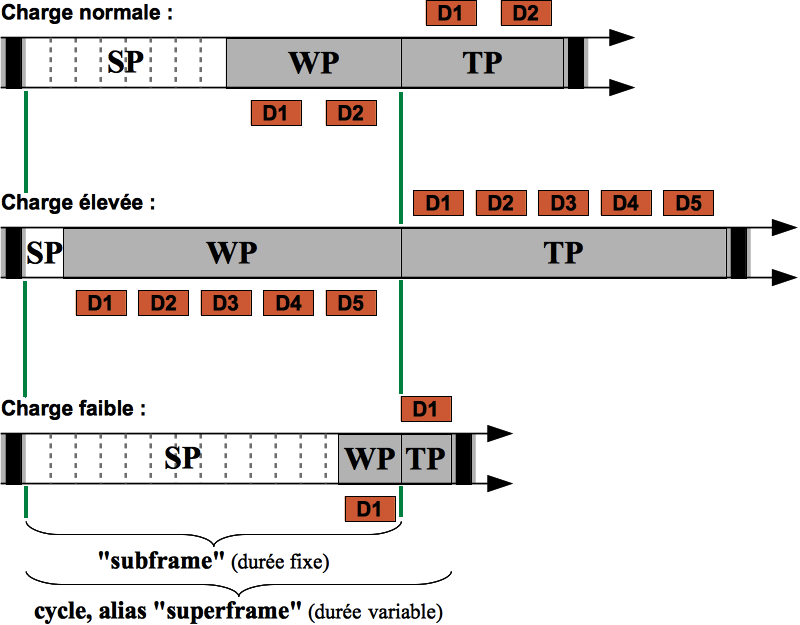
\includegraphics[width=10cm]{images/ch3-s-cosens-cycle.png}
\flcaption{Principe d'un cycle de fonctionnement d'un noeud coordinateur
S-CoSenS. (Source~: \cite{TheseBNefzi})}
\label{FigCycleSCoSenS}
\end{figure}

Cette synchronisation locale au sein d'un PAN S-CoSenS, faite grâce
à l'envoi cyclique d'un \lang{``beacon''}, repose donc sur le paradigme
LPP (\lang{Low Power Probing}, principe détaillé plus haut). D'un
autre côté, la synchronisation et la communication entre routeurs
S-CoSenS appartenant à des PANs différents se fait grâce à de courtes
périodes d'éveil et d'écoute se déroulant durant la période de sommeil
(SP), et repose donc sur le paradigme LPL (\lang{Low Power Listening},
comme pour X-MAC par exemple), pour des raisons de simplicité.

À noter que le cycle S-CoSenS complet (SP + WP + TP) ne concerne que
les noeuds jouant le rôle de routeur et de coordinateur de PAN.

En effet, une propriété intéressante de S-CoSenS est que les noeuds
terminaux ou noeuds-feuilles (c'est-à-dire ceux n'ayant pas un rôle de
routeur ou de coordinateur de réseau) peuvent garder leur émetteur~/
récepteur radio constamment éteint, tant qu'ils n'ont pas de trame
à envoyer. Quand un de ces noeuds-feuilles doit envoyer une trame de
données, il démarre sa radio, écoute et attend le premier \lang{``beacon''}
émis par un routeur, puis émet sa trame en utilisant la méthode
CSMA/CA au début de la période de réception (WP) annoncée dans le
\lang{``beacon''} qu'il a reçu. Ce noeud-feuille peut éteindre sa radio
pendant le délai courant entre le \lang{``beacon''} et la WP attendue
(c'est-à-dire durant le délai correspondant à la période de sommeil
SP du routeur ayant émis le \lang{``beacon''}), émet sa trame durant
la WP voulue, puis peut retourner à l'état de sommeil une fois sa
trame transmise avec succès.

Toute cette procédure de transmission est résumée dans la figure
\vref{FigSCoSenSTransmission}. Dans cette figure, les parties grises
représentent les périodes où un noeud fait fonctionner sa radio,
les blocs oranges correspondent aux transmissions de trames, tandis que
les parties blanches sont celles où le noeud met sa radio en sommeil pour
économiser son énergie. Le noeud simple émetteur se réveille quand une
trame doit être émise, attend le \lang{``beacon''} issu du routeur,
se synchronise alors pour émettre la trame durant la période de réception
(WP) du routeur, puis retourne en mode sommeil. Le routeur peut ensuite
réemettre la trame vers la destination adéquate durant sa période
de transmission (TP).

\begin{figure}[!hbt]
\centering
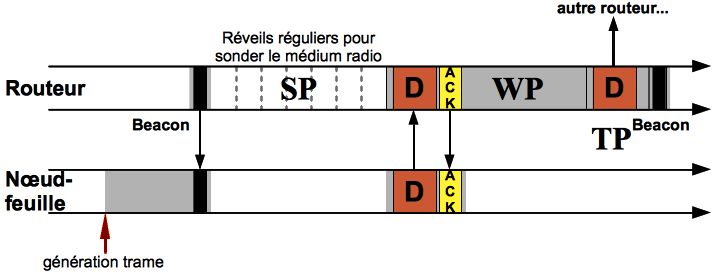
\includegraphics[width=9.5cm]{images/ch3-s-cosens-transmission.png}
\flcaption{Transmission d'une trame avec le protocole S-CoSenS.}
\label{FigSCoSenSTransmission}
\end{figure}

\bigskip

Si ce protocole représente une amélioration certaine par rapport
au protocole MAC de base du standard 802.15.4 et aux protocoles
LPL et LPP classiques~--- comme nous le verrons dans le chapitre
\ref{ChProtocolesMAC} de la présente thèse~---, il continue néanmoins
de souffrir des limitations intrinsèques liées au principe de contention
sur lequel il est basé~: lors de trafics réseaux intenses, la qualité
de service (taux de trames transmises avec succès, délais de
transmission) chute irrémédiablement. Ces problèmes sont mieux
pris en charge par les protocoles basés sur l'ordonnancement
(TDMA) mais ceux-ci posent d'autres problèmes (complexité,
lourdeur d'organisation). Des recherches ont donc été menées
pour contourner ces problèmes, et ont abouti à la mise au
point de nouveaux protocoles plus performants, dont celui
que nous allons maintenant détailler dans la section
\ref{PariQueueMAC} suivante.

\subsubsection{iQueue-MAC}
\label{PariQueueMAC}

Ce protocole, de conception récente et ambitieuse \cite{iQueueMAC}, est un
protocole ordonnancé hybride, utilisant la contention (méthode CSMA/CA)
et l'ordonnancement temporel (TDMA) en fonction du trafic réseau courant.

Nous avons vu en effet plus haut qu'il a été démontré que la méthode CSMA
est plus efficace pour le traitement des faibles trafics, tandis que TDMA
est nettement plus appropriée pour supporter les trafics intenses.

Si le protocole MAC standard 802.15.4 en <<~mode \lang{``beacon''}~>> fait
déjà appel à une approche hybride (avec les notions de CAP et CFP), il est
limité par la configuration totalement statique de ses paramètres de
fonctionnement.

À l'inverse, iQueue-MAC est conçu pour s'adapter dynamiquement et en
temps réel au trafic du réseau, de façon à adopter à chaque instant la
meilleure configuration pour optimiser qualité de service et consommation
d'énergie (via la maîtrise du \lang{duty cycle} et de ses différentes
périodes, dont les durées sont dynamiques).

La figure \vref{FigiQueueMACCharge} montre comment iQueue-MAC gère la
montée en charge du trafic réseau de façon totalement différente d'autres
protocoles plus classiques basés sur la seule contention (comme par exemple
S-CoSenS).

\begin{figure}[!hbt]
\centering
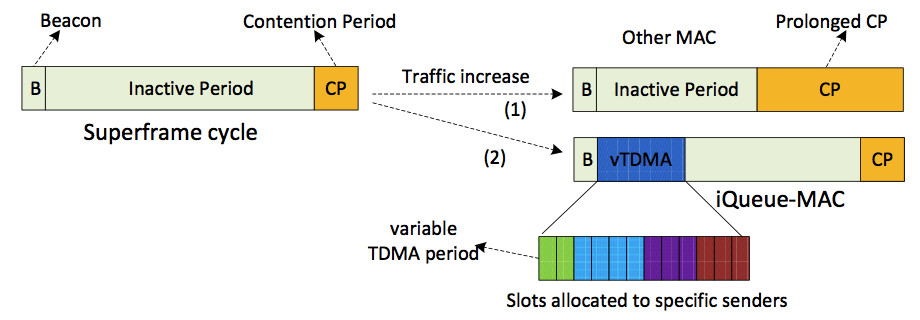
\includegraphics[width=12.5cm]{images/ch3-iqueue-mac-charge.png}
\flcaption{Comparaison de la gestion de la montée en charge du trafic
réseau entre \textbf{(1)}~un protocole uniquement basé sur la contention,
et \textbf{(2)}~iQueue-MAC, qui a recours à une période basée sur TDMA
de durée variable, adaptée à la charge réseau.
(Source~: \cite{coursEnsem})}
\label{FigiQueueMACCharge}
\end{figure}

Les idées principales qui sous-tendent la conception d'iQueue-MAC sont
les suivantes~:
\begin{itemize}
\item L'utilisation de la contention (CSMA/CA) quand le trafic est faible,
et de l'ordonnancement temporel (TDMA) quand le trafic devient intense.
\item La séparation des noeuds sans-fil en deux catégories~: les noeuds
simples (terminaux ou noeuds-feuilles) et les routeurs.
\item Les noeuds simples (tout comme avec la famille CoSenS) ne s'éveillent
que quand ils ont des données à envoyer, et passent donc la majeure partie
de leur temps en sommeil pour économiser leur énergie.
\item Les routeurs sont les noeuds exécutant véritablement la totalité
du mécanisme d'iQueue-MAC.
\item Le protocole base son comportement et sa configuration sur la
connaissance de la quantité de trames à envoyer (c'est-à-dire la
longueur de la file d'envoi de trames) pour chaque noeud du réseau.
\end{itemize}

En effet, chaque noeud simple, lorsqu'il envoie une trame, insère le
niveau d'occupation de sa file d'envoi (juste après l'entête de la trame).
Le routeur est donc à chaque cycle capable d'évaluer la charge que
devra soutenir le réseau lors du cycle suivant. La structure d'une
trame iQueue-MAC est représentée figure \vref{FigiQueueMACTrame}.
On notera l'ajout du taux d'occupation de la file d'envoi du noeud émetteur
entre l'entête MAC et la charge utile (\lang{``payload''}) de la trame
proprement dite.

\begin{figure}[!bpt]
\centering
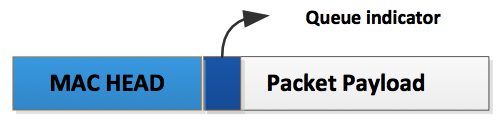
\includegraphics[width=7.5cm]{images/ch3-iqueue-mac-paquet.png}
\flcaption{Structure d'une trame iQueue-MAC.
(Source~: \cite{coursEnsem})}
\label{FigiQueueMACTrame}
\end{figure}

Chaque cycle iQueue-MAC (également appelé \nom{superframe}, est
représenté figure \vref{FigiQueueMACCycle}. La \lang{subframe} est
la partie du cycle dont la durée est calculée (donc connue) à l'avance~;
elle comporte la période TDMA, dont la durée varie en fonction de
l'intensité du trafic réseau, et dont les \lang{slots} temporels
sont alloués aux différents noeuds en fonction de la quantité
de trames qu'ils ont à émettre (ces quantités ayant été transmises
durant la période de contention du cycle précédent).

Un cycle iQueue-MAC se décompose donc en les phases suivantes~:
\begin{description}
\item[B~: \lang{``beacon''}.]
Celui-ci permet la synchronisation des différents noeuds du PAN~:
il indique la durée et l'affectation des différents \lang{slots} de la
période TDMA, ainsi que la durée de la période de sommeil. L'ensemble
regroupant les slots de temps TDMA et la période de sommeil est appelé
\emph{subframe}~: c'est la partie du cycle iQueue-MAC dont la durée est
calculée et allouée à l'avance. La structure d'un \lang{``beacon''}
iQueue-MAC est détaillée figure \vref{FigiQueueMACBeacon}.
Toutes les données nécessaires pour calculer la durée de la
\lang{subframe}, de la section TDMA variable, et l'allocation
des différents \lang{slots} de temps TDMA aux différents noeuds
demandeurs sont présentes.

\begin{figure}[!bpt]
\centering
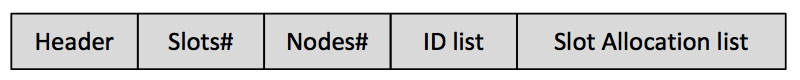
\includegraphics[width=9cm]{images/ch3-iqueue-mac-beacon.png}
\flcaption{Structure d'un \lang{``beacon''} iQueue-MAC.
(Source~: \cite{coursEnsem})}
\label{FigiQueueMACBeacon}
\end{figure}

\item[SF~: \lang{SubFrame}]
Cette période contient les slots de temps TDMA dont l'allocation aux
différents noeuds a été annoncée dans le \lang{``beacon''}~; ces slots TDMA
sont suivis de la période de sommeil où la radio du routeur est éteinte
pour économiser l'énergie. Notons que comme dans d'autres protocoles tels
que X-MAC ou S-CoSenS, de courts moments d'activation de la radio ont lieu
durant la période de sommeil, afin de pouvoir détecter et recevoir des
messages en provenance de routeurs d'autres PANs.
\item[CP~: \lang{Contention Period}]
Période de réception basée sur le principe de la contention (CSMA/CA) où
chaque noeud du PAN est autorisé à transmettre une et une seul trame~---
s'il a plus d'une trame de données à transmettre, l'indicateur de
remplissage de sa file d'envoi situé au début de la charge utile
(\lang{``payload''}) de la trame lui fera allouer le nombre de \lang{slots}
nécessaires durant la \lang{subframe} du cycle suivant. La durée de la CP
n'est pas prédéterminée~: le routeur écoute jusqu'à la survenue d'un
\lang{timeout} d'inactivité radio, ce qui est censé donner assez de temps
à chaque noeud ayant des données à émettre (principe similaire à celui
vu plus haut pour T-MAC).
\item[TP~: \lang{Transmission Period}]
La retransmission des trames par le routeur~--- vers le routeur suivant
ou le concentrateur final~/ station de base du réseau sans fil
(\lang{``sink''})~--- se fait par lots (en mode \lang{``burst''}),
comme par exemple pour les protocoles T-MAC ou RI-MAC vus plus haut~:
une fois la première trame envoyée avec succès, les trames suivantes
sont envoyées avec un minimum \lang{d'overhead}.
\end{description}

\begin{figure}[!bpt]
\centering
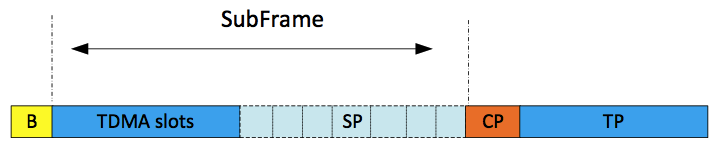
\includegraphics[width=12cm]{images/ch3-iqueue-mac-cycle.png}
\flcaption{Structure d'un cycle iQueue-MAC.
(Source~: \cite{coursEnsem})}
\label{FigiQueueMACCycle}
\end{figure}

\begin{figure}[!htb]
\centering
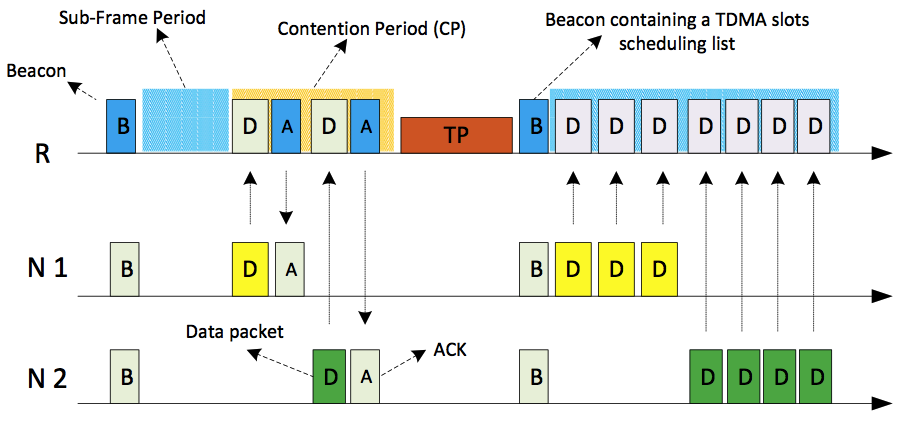
\includegraphics[width=12cm]{images/ch3-iqueue-mac-exemple-transmission.png}
\flcaption{Exemple de transmission de trames entre deux noeuds simples
et un routeur avec le protocole iQueue-MAC.
(Source~: \cite{coursEnsem})}
\label{FigiQueueMACExemple}
\end{figure}

\newpage

Donnons ici un exemple de déroulement d'une transmission d'un lot
de trames depuis deux noeuds simples vers un routeur iQueue-MAC,
tel que montré dans la figure \vref{FigiQueueMACExemple}~:
\begin{enumerate}
\item Soit un routeur R, et deux noeuds N1 et N2, ayant respectivement
4 et 5 trames de données à transmettre~; on suppose qu'aucune autre
transmission n'est en cours à ce moment-là dans ce PAN.
\item Pendant le premier cycle, N1 et N2 reçoivent le \lang{``beacon''}
de synchronisation. Aucun slot TDMA n'étant alloué, ils attendent tous
deux la période de contention CP, et émettent chacun leur première trame
de données~; la méthode CSMA/CA étant utilisée, ils reçoivent un
acquittement pour l'envoi de ces premières trames.
\item Le routeur termine son cycle par sa période de transmission TP,
et le premier cycle se termine.
\item Le routeur ayant reçu la taille des files d'envoi des deux
noeuds lors de la période de contention précédente, il alloue donc
le nombre de \lang{slots} TDMA nécessaire aux différents noeuds~:
3 pour N1, et 4 pour N2. Une fois les durées nécessaires calculées,
le second cycle commence, et un nouveau \lang{``beacon''} est envoyé.
\item Les noeuds N1 et N2 reçoivent ce \lang{``beacon''} et se synchronisent
pour l'envoi de leurs données durant la \lang{subframe}
\item Les trois premiers \lang{slots} TDMA étant alloués à N1, celui
envoie dès le début de la \lang{subframe} ses trames restantes. Sa file
d'envoi étant désormais vidée, il peut retourner en mode sommeil, jusqu'à
ce qu'il ait par la suite de nouvelles données à envoyer.
\item Les quatre \lang{slots} TDMA suivants étant alloués à N2, il
peut lui aussi envoyer à son tour les trames de données restant dans sa
file d'envoi, et à son tour passer en mode sommeil pour économiser son
énergie.
\item Toutes les données ayant besoin d'être transmises sont désormais
arrivées au routeur, qui peut terminer sa \lang{subframe} en période
de sommeil, puis retransmettre ces trames de façon adéquate durant
la période de transmission (TP) qui terminera ce second cycle (mais
n'est pas montrée sur la figure \vref{FigiQueueMACExemple}).
\end{enumerate}

\medskip

Les différentes expériences menées dans la publication \cite{iQueueMAC}
ont montré la nette supériorité d'iQueue-MAC en termes de qualité de
service~--- taux de trames transmises avec succès, délai total de
transmission~--- dans toutes les configurations, vis-à-vis de protocoles
tels que RI-MAC ou CoSenS (lequels avaient eux-mêmes déjà prouvé leur
supériorité sur les protocoles LPL classiques couramment utilisés).
Cette supériorité est notamment flagrante pour les charges réseaux intenses,
ou pour le traitement de pics soudains de trafic. Ce protocole semble donc
se poser en concurrent sérieux pour le nouveau protocole 802.15.4e~;
ce dernier ayant pour avantage sa capacité de traitement multicanal, tandis
que iQueue-MAC semble plus à même d'exploiter au mieux le débit maximal
théorique d'une unique fréquence radio, ce qui rend sa conception
et son implantation plus simple~--- avantage non négligeable lorsqu'il
s'agit d'implanter un protocole MAC sur un appareil à fonctionnalités
limitées (<<~RFD~>> standard IEEE 802.15.4).

\subsubsection{Autres évolutions de protocoles basés sur la contention}
\label{ParProtoTNoel}

Outre les protocoles avancés développés par notre équipe que nous avons
décrit ci-dessus dans les sections \vrefrange{ParSCoSenS}{PariQueueMAC},
d'autres équipes de recherche continuent également d'apporter de
nouvelles idées et techniques pour améliorer les performances et/ou
diminuer la consommation énergétique des protocoles MAC~/ RDC.

\smallskip

Nous citerons ici, à titre d'exemple, les travaux menés à l'Université
de Strasbourg pour améliorer les protocoles basés sur la technique LPL,
grâce notamment à un mécanisme nommé T-AAD (\lang{lightweight ``Traffic
Auto-ADaptations''} \cite{T-AAD}, conçu pour permettre aux protocoles LPL
de mieux gérer les pointes (\lang{``bursts''} de trafic réseau.

Le mécanisme \nom{T-AAD} consiste à adapter automatiquement les paramètres
des protocoles MAC dynamiquement en fonctions des variations du trafic
réseau. Le principal paramètre d'un protocole LPL étant la durée de la
période de sommeil (ici appelée $ST$) entre deux CCA consécutifs~---
c'est-à-dire en fait la durée du cycle de ces protocoles LPL~---,
T-AAD se propose d'alterner la durée de $ST$ entre deux extremums,
$ST_{min}$ et $ST_{max}$, selon la charge réseau. $ST_{max}$ est la durée
de cycle longue (par exemple, 500~ms), employée par défaut, lorsque la
charge réseau est à son niveau <<~de base~>>. $ST_{min}$ est la durée
de cycle courte (par exemple, 32~ms), utilisée temporairement afin
de prendre en charge efficacement les pointes de trafic réseau.

Afin de pouvoir estimer dynamiquement la charge réseau à venir, T-AAD
impose à chaque noeud d'ajouter, à chaque paquet émis, le nombre de paquets
lui restant à émettre dans sa file d'envoi. Un noeud récepteur employant
T-AAD utilise alors cette information pour calculer le temps durant lequel
il va passer sa durée de cycle à $ST_{min}$ pour gérer cette charge à venir~:
cette durée de fonctionnement <<~intensif~>> est nommée $T_{adapt}$.
Une fois la durée $T_{adapt}$ écoulée, le noeud revient à la durée de cycle
par défaut $ST_{max}$. (Notons que quand un noeud émetteur n'émet qu'une
charge réseau modérée, $T_{adapt}$ sera calculée à la valeur 0, et
le récepteur gardera alors un cycle standard de durée $ST_{max}$.)

Le but du mécanisme T-AAD est donc de rendre les protocoles LPL
<<~classiques~>> (comme X-MAC ou ContikiMAC) auto-adaptatifs à la charge
réseau, comme le sont naturellement CoSenS~/ S-CoSenS et iQueue-MAC.

Notons toutefois qu'il s'agit d'un mécanisme bien plus simple que pour
nos deux protocoles, la durée de cycle variant de façon discrète entre
deux valeurs, et non de façon continue et précise. L'avantage de T-AAD
est d'être ainsi d'une conception bien plus simple, au prix d'une
moindre précision dans l'adaptation de la durée des cycles MAC~;
toutefois, comme ce mécanisme doit s'adapter à des protocoles n'ayant
pas été au départ conçus pour être auto-adaptatifs, une telle simplicité
peut être considérée comme mieux adaptée à la cible choisie.

\medskip

Ce mécanisme T-AAD a été implémenté et testé pour améliorer des
protocoles LPL classiques comme X-MAC \cite{T-AAD} \cite{T-AAD-demo}
(se reporter respectivement à la section \vref{ParXMAC} pour les détails
sur le fonctionnement <<~standard~>> de ce protocole). Les changements
apportés par le mécanisme T-AAD dans le fonctionnement de X-MAC sont
illustrés dans la figure \vref{Fig-TAAD-XMAC}.

\begin{figure}[!htb]
\centering
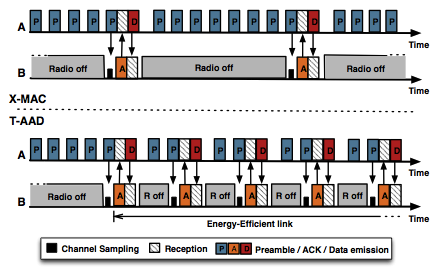
\includegraphics[width=11cm]{images/ch3-t-aad-x-mac.png}
\flcaption{Modification du fonctionnement du protocole X-MAC par le
mécanisme T-AAD. (Source~: \cite{T-AAD})}
\label{Fig-TAAD-XMAC}
\end{figure}

Il a été montré dans \cite{T-AAD} que ce mécanisme simple~--- donc
relativement facile à implémenter et peu coûteux en occupation mémoire
et en temps processeur~--- a permis d'améliorer significativement les 
performances (notamment en termes de délais de transmission) et
l'efficacité énergétique du protocole X-MAC ainsi modifié. Ces améliorations
ont été constatées par des tests faits sur du matériel réel, à savoir~:
les noeuds du \lang{testbed} IoT-LAB \cite{IotLAB}.

\bigskip

Plus récemment, cette même équipe a publié plusieurs versions améliorées
de ContikiMAC (cf. section \ref{ParContikiMAC} pour plus de détails sur
ce protocole MAC~/ RDC), destinées à être mieux adaptées aux noeuds mobiles,
nommées M-ContikiMAC et ME-ContikiMAC \cite{ME-ContikiMAC} (M signifiant ici
\lang{``Mobile''}, et ME \lang{``Mobile Enhanced''}.

Le protocole \nom{M-ContikiMAC} consiste à utiliser pour émettre ses trames
un mode de transmission \lang{``anycast''}, permettant à n'importe quel
noeud à portée de recevoir un paquet. Contrairement toutefois au mode
\lang{``broadcast''} que nous avons vu pour l'envoi de \lang{``beacons''},
en mode \lang{``anycast''} tout récepteur est tenu de renvoyer un paquet
d'acquittement, comme pour une transmission classique (également appelée
\lang{``unicast''}. Une fois un ou plusieurs récepteurs identifiés grâce
aux premiers envois de paquets en mode \lang{``anycast''}, les transmissions
suivantes de trames peuvent se faire de façon classique \lang{``unicast''}
suivant le mécanisme standard de ContikiMAC. Ce mode opératoire, bien
adapté aux noeuds mobiles ne pouvant compter sur des protocoles de routage
avancés pour découvrir leur entourage, peut être illustré grâce au schéma
montré en figure \vref{FigMContikiMAC} (où un noeud mobile communique
avec un noeud fixe parmi deux présents dans un WSN donné).

\begin{figure}[!htb]
\centering
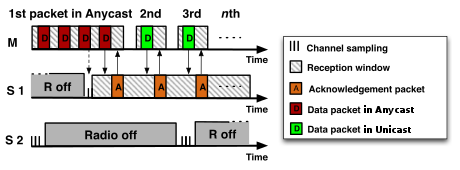
\includegraphics[width=10.75cm]{images/ch3-m-contikimac.png}
\flcaption{Fonctionnement du protocole avancé M-ContikiMAC, optimisé pour
les noeuds mobiles des WSN. (D'après \cite{ME-ContikiMAC})}
\label{FigMContikiMAC}
\end{figure}

\medskip

Sur la base de M-ContikiMAC, la même équipe a alors ensuite développé
\nom{ME-ContikiMAC}. Ce dernier protocole a notamment été conçu pour mieux
gérer les problèmes liés à la duplication des paquets et à l'optimisation
des délais de transmission, par rapport à M-ContikiMAC. Pour ce faire,
ME-ContikiMAC envoie désormais en \lang{``anycast''}, pour chercher
des récepteurs et établir des <<~connexions~>>, non plus des trames
de données (comme dans ContikiMAC), mais des trames de contrôle, dont
l'émission est maintenue même en cas de collision au niveau des paquets
d'acquittement, jusqu'à la réception d'un paquet d'acquittement correct.
L'envoi des trames de données se fait ensuite uniquement en
\lang{``unicast''}, jusqu'à la fin de la transmission ou la <<~perte
de connexion~>> (par exemple quand le noeud mobile n'est plus à portée).

Le fonctionnement de ME-ContikiMAC peut être illustré par la figure
\vref{FigMEContikiMAC}. On y voit notamment la façon dont ce protocole
gère les collisions et la déduplications de paquets, et ce avec
un noeud mobile communicant avec trois noeuds fixes.

\begin{figure}[!hbt]
\centering
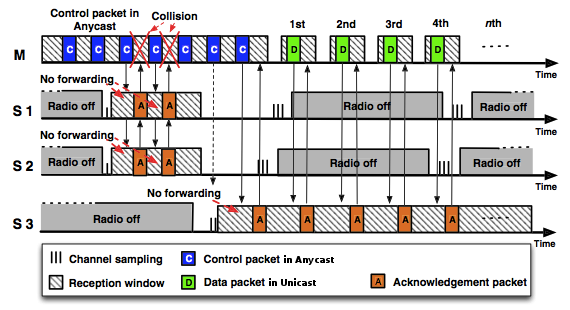
\includegraphics[width=12.75cm]{images/ch3-me-contikimac.png}
\flcaption{Fonctionnement du protocole avancé ME-ContikiMAC.
(D'après \cite{ME-ContikiMAC})}
\label{FigMEContikiMAC}
\end{figure}

Là encore, l'article \cite{ME-ContikiMAC} montre des améliorations
sensibles au point de vue de la qualité de service (déduplication de
paquets, occupation du médium radio, delais de transmissions réduits)
et de la consommation énergétique. ME-ContikiMAC a notamment montré,
dans ladite publication, que ces améliorations étaient sensibles vis-à-vis
de WSN ayant des noeuds statiques mais aussi et surtout des noeuds
mobiles. (Notons toutefois que cet article ne s'appuie, contrairement
aux publications sur T-AAD, que sur des simulations effectuées sous
Cooja).

\bigskip

On voit donc au final que de nombreuses équipes de recherches continuent
à explorer continuellement et activement de nombreuses pistes pour
améliorer les couches MAC~/ RDC des piles protocolaires des WSN,
que ce soit par la conception de protocoles entièrement nouveaux~---
tels CoSenS~/ S-CoSenS et iQueue-MAC~--- ou par l'invention de mécanismes
astucieux et efficaces pour améliorer les protocoles existants.

Les deux approches peuvent l'une comme l'autre permettre d'obtenir
des résultats significatifs en termes d'optimisation de la qualité
de service et de la consommation d'énergie. 

\subsubsection{Approches multi-couches~: l'exemple de la pile OCARI}
\label{ParOCARI}

Outre le seul développement de protocoles MAC~/ RDC~--- c'est-à-dire
de solutions relevant exclusivement de la couche 2 du modèle OSI~---,
plusieurs travaux consistant en le développement de piles protocolaires
complètes, pouvant aller jusqu'aux couches du plus haut niveau, ont été
menés. On peut noter que de tels travaux ont été menés plus souvent dans
un cadre industriel que dans celui de la recherche purement académique,
comme c'était majoritairement le cas des protocoles que nous avons vu
jusqu'ici dans cet état de l'art.

De telles approches, dites <<~multi-couches~>> ou \lang{``cross-layer''},
incluent donc une couche MAC qui, par définition, est intimement liée
au reste de la pile, et n'est \lang{a priori} pas conçue pour être
implantée de façon indépendante.

Un exemple d'une telle pile protocolaire complète, basé sur la couche
physique du standard IEEE 802.15.4 (sur la bande à 2,4~GHz uniquement)
est OCARI (Optimisation des Communications Ad-hoc pour les Réseaux
Industriels) \cite{OCARI}. Comme son nom l'indique, il s'agit ici d'un
effort de rechcerche appliquée~--- mené par une alliance regroupant
différents acteurs majeurs, industriels et académiques~--- destiné à
fournir une pile réseau à très haute fiabilité, afin d'offrir une
solution pour des applications critiques comme celles liées aux
centrales nucléaires ou aux navires militaires.

De cet effort est née une pile protocolaire complète, allant de la couche
MAC~/ RDC (niveau 2 OSI) aux API destinées à la programmation d'applications
(assimilable au niveau 7 OSI). Compte-tenu du sujet de notre thèse, nous
nous cantonnerons à l'étude de la couche MAC, nommée \nom{MaCARI}, bien que
celle-ci soit étroitement liée aux autres couches d'OCARI. Cette couche
est notamment prévue pour faciliter les opérations de routage, en
coopération étroite avec les couches supérieures d'OCARI.

L'organisation d'un cycle MaCARI se divise en trois périodes, et est
représentée sur la figure \vref{FigMaCARICycle}.

\begin{figure}[!htb]
\centering
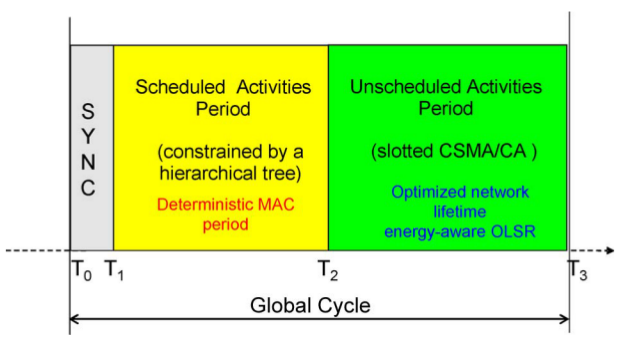
\includegraphics[width=10cm]{images/ch3-ocari-macari-cycle.png}
\flcaption{Structure d'un cycle du protocole MaCARI.
(Source~: \cite{OCARI} figure 3)}
\label{FigMaCARICycle}
\end{figure}

\smallskip

Ces trois périodes sont~:
\begin{enumerate}
\item une période de synchronisation des différents noeuds ($T_0$--$T_1$),
en gris sur la figure \vref{FigMaCARICycle}~;
\item une période de transmissions pré-déterminées ($T_1$--$T_2$), basée
sur une méthode TDMA optimisée, assurant une réservation de \lang{slots}
dépourvue de toute interférence pour toute transmission, en jaune sur
la  figure \vref{FigMaCARICycle}~;
\item une période de transmissions <<~spontanées~>> ($T_2$--$T_3$), basée
sur la contention (CSMA/CA slottée), en vert sur la figure
\vref{FigMaCARICycle}.
\end{enumerate}

Le protocole MaCARI est véritablement un protocole hybride, puisque l'on
peut le considérer à la fois comme un protocole synchrone, un protocole basé
sur le multiplexage temporel (TDMA), et un protocole basé sur la contention.
Il s'agit enfin d'un protocole MAC~/ RDC, l'émetteur~/ récepteur radio
pouvant être mis hors fonction pour économiser l'énergie durant la période
<<~déterministe~>> quand un noeud n'a pas à communiquer durant son
\lang{slot} assigné.

Si le protocole MaCARI est, comme on le voit, très performant et ingénieux,
son intégration étroite avec le reste de la pile OCARI~--- le rendant
délicat à porter et utiliser indépendamment de cette pile~--- et son
orientation très industrielle ne lui ont jusqu'ici pas permis d'apparaître
dans des OS spécialisés pour WSN comme Contiki~; de plus, la présence d'une
pile fournissant un ensemble très complet de fonctionnalités, pouvant
presque faire doublon avec un système d'exploitation proprement dit,
rend un tel portage encore plus difficile.

Rappelons enfin que les piles protocolaires complètes étant au-delà du sujet
de la présente thèse, nous n'avons au cours de celle-ci effectué aucun
travail avec ce protocole.


\subsection{Discussion~: les protocoles MAC~/ RDC}
\label{SubsecDiscussMAC}

En sus de l'évolution du protocole IEEE 802.15.4, et pour tenter de
dépasser les limitations de celui-ci, la recherche académique a depuis
maintenant plus d'une douzaine d'années proposé de nombreux protocoles
MAC alternatifs. Comme nous venons de le voir, plusieurs approches
ont été explorées~: protocoles basés sur la contention~--- qu'ils soient
synchrones ou asynchrones, ces derniers pouvant être basés sur
l'initiation des transmissions par les noeuds émetteurs (LPL) ou
par les noeuds récepteurs (LPP)~---, protocoles basés sur l'ordonnancement
par multiplexage temporel (TDMA) ou fréquentiel (FDMA) des transmissions.
Enfin, des protocoles hybrides, exploitant plusieurs de ces approches,
ont plus récemment été publiés~: nous avons présenté deux de ces
protocoles conçus par notre équipe, et l'amendement 802.15.4e du
standard IEEE repose lui-même sur une utilisation simultanée des
deux techniques de multiplexage temporel et fréquentiel.

Toutes ces approches ont été explorées au cours du temps par diverses
équipes. Notre présentation dans la présente section est, comme nous
l'avons signalé, loin d'être exhaustive, et la figure \vref{FigTaxonomieMAC}
reprise de l'article de référence de \cite{Evolution-MAC-WSN-Survey-2013}
montre l'intense activité de recherche ayant eu lieu dans ce domaine.
(Il faut de plus ajouter que cette figure date de fin 2011, et
ne prend pas en compte les développements les plus récents,
comme l'amendement 802.15.4e du standard IEEE.)

\begin{figure}[!htb]
\centering
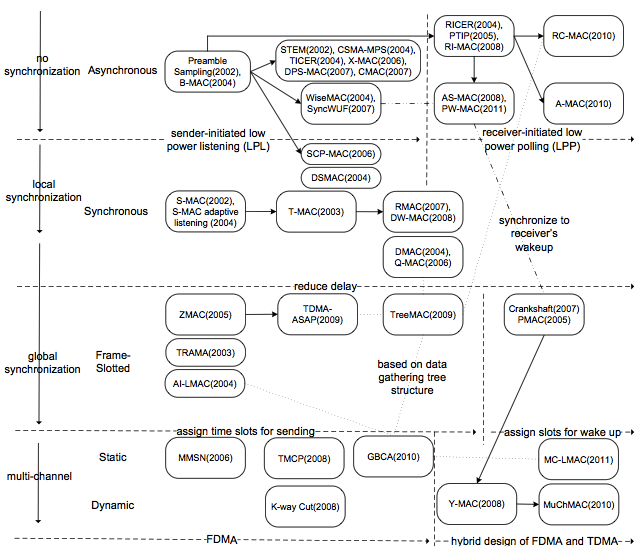
\includegraphics[width=12.5cm]{images/ch3-taxonomie-mac.png}
\flcaption{Taxonomie des différents protocoles MAC conçus pour
les réseaux de capteurs sans-fil (travaux académiques).
Source~: \cite{Evolution-MAC-WSN-Survey-2013}}
\label{FigTaxonomieMAC}
\end{figure}

Pour le moment, et malgré tous ces développements, les protocoles
asynchrones LPL restent, du moins dans le milieu académique, les plus
couramment utilisés. Ils sont en effet bien adaptés aux trafics réseaux
modérés, ce qui correspond au mode de fonctionnement de la majorité des
réseaux de capteurs sans-fil à l'heure actuelle, et permettent à la fois
une bonne économie des ressources, tant du point de vue énergétique
(économie de la batterie des noeuds) que matériel (simplicité
d'implantation, d'où une faible occupation de la mémoire~--- d'une
capacité souvent extrêmement limitée~--- de ces appareils).
Le protocole ContikiMAC, grâce à la forte influence du système
d'exploitation Contiki dans le domaine des réseaux de capteurs
sans-fil (comme nous allons le voir dans la section \vref{SecOSWSN})
tend actuellement à devenir le standard de fait dans les différents
travaux de recherche dans le domaine.

Toutefois, l'adoption de l'amendement 802.15.4e au standard IEEE,
avec sa couche MAC évoluée (mécanisme TSCH) et le développement d'une
pile réseau complète sur cette base (projet 6TiSCH \cite{6TiSCH}
\cite{6TiSCHbis} \cite{6TiSCHter}) pourraient prochainement changer
la donne, et imposer un nouveau standard notamment dans les réseaux
industriels exigeants~--- surtout ceux composés de noeuds puissants
pouvant jouer le rôle de FFD (\lang{``Full Function Devices''}).
Le développement de la pile réseau avancée OpenWSN est un autre facteur
susceptible de faciliter une telle évolution.


%%%%%%%%%%%%%%%%%%%%%%%%%%%%%%%%%%%%%%%%%%%%%%%%%%%%%%%%%%%%%%%%%%%%%%%%%%%%%

\section{Systèmes d'exploitation dédiés}
\label{SecOSWSN}

Des systèmes d'exploitation spécialisés pour les appareils embarqués
spécifiques que sont les noeuds des réseaux de capteurs sans-fils
(les \lang{``motes''}) ont été conçus et publiés depuis maintenant
plus d'une dizaine d'années.

Rappelons que pour des raisons juridiques aussi bien que techniques~---
possibilité de modifier et d'améliorer le c{\oe}ur et les différents
composants du système selon nos besoins~--- nous n'avons étudié et
envisagé l'utilisation que des systèmes à licence libre et \lang{open
source}.

\subsection{Rappels sur les notions de multi-tâche}
\label{SubsecMultitache}

\`A un moment donné, un micro-contrôleur (du moins la majorité d'entre eux,
qui ne disposent que d'un unique <<~c{\oe}ur~>>) ne peut exécuter qu'une
tâche à la fois. Pour qu'un système informatique, comme une \lang{mote},
puisse effectuer plusieurs tâches, il est nécessaire de passer régulièrement
et très rapidement d'une de ces tâches à une autre. Cela introduit la notion
de \emph{changement de contexte}~: lorsqu'on passe d'une tâche A à une
autre tâche B, on sauvegarde l'état de A pour charger celui de B~;
l'état d'une tâche étant nommé son \nom{contexte} (il s'agit des valeurs
des registres du processeur, des périphériques, etc.)

L'espace où sont sauvegardés les contextes des différentes tâches est nommé
\emph{pile} (en anglais~: \lang{``stack''}). Il s'agit d'une structure
de données variable située en mémoire (RAM donc), suivant le paradigme
<<~dernier entré, premier sorti~>> (en anglais LIFO~: \lang{Last In
First Out}).

Notons que la pile n'est pas dédiée aux seuls contextes de tâches~:
elle sert également de zone de travail en mémoire pour les programmes
en cours d'exécution (variables locales, appels de sous-programmes, etc.)

Selon la conception du système d'exploitation, il peut y avoir une seule
pile commune à tout le système, ou plusieurs piles dédiées aux différentes
tâches, comme nous allons le voir.

On distingue deux principaux modèles conceptuels pour réaliser un système
multi-tâche~:

\begin{description}

\item[le multi-tâche coopératif~:] dans ce modèle, chaque tâche doit prévoir
explicitement dans son  code source de <<~passer la main~>> (par l'appel à
une fonction dédiée du système d'exploitation).
Ce modèle rend les systèmes d'exploitation plus simples à concevoir et
plus compacts~: il est en effet possible dans ce cas d'employer une pile
unique pour l'ensemble du système.
En contrepartie, la programmation d'applications est plus contraignante~:
le développeur doit gérer lui-même le basculement d'une tâche à une autre,
sinon le système est condamné à mal fonctionner, et même en général à se
bloquer (<<~se planter~>>). Ce modèle rend donc au final le système moins
robuste~: une tâche mal programmée (par exemple~: ne passant pas la main)
peut mettre tout le système hors service.

\item[le multi-tâche préemptif~:] dans ce modèle, le système d'exploitation
alloue lui-même les intervalles d'exécution à chaque tâche, et planifie
automatiquement les changements de contexte entre celles-ci (cette capacité
d'interrompre une tâche sans collaboration de sa part est nommée
\nom{préemption}). Ce modèle implique des systèmes d'exploitation plus
évolués et gourmands en ressources~: il est en effet nécessaire d'avoir une
pile distincte par tâche. En contrepartie, la programmation d'applications
est nettement simplifiée~: le développeur n'a pas à se soucier des
changements de tâches. Le système est en outre nettement plus robuste~:
une tâche « bloquée » ne va pas systématiquement mettre hors service
tout le système.

En outre, la capacité d'interrompre à n'importe quel moment une tâche
en cours est un pré-requis pour implanter un système temps réel, qui
a besoin de pouvoir réagir à un évènement comme une interruption en un délai
limité. C'est pourquoi les systèmes offrant des fonctionnalités temps-réel
sont basés sur le modèle préemptif, le multi-tâche coopératif~---
qui oblige à attendre que la tâche en cours soit prête à passer la main~---
étant par conception défavorable à ces fonctionnalités.\\
Cela est illustré par la figure \vref{FigModeleMultitache}.
On notera notamment la latence présente en modèle coopératif \textbf{A}
due à l'attente de la fin de la tâche en cours, absente du modèle préemptif
\textbf{B} pouvant interrompre une tâche à tout moment (sauf à être
déjà en train de gérer un évènement ou une interruption).

\end{description}

\begin{figure}[!hbt]
\centering
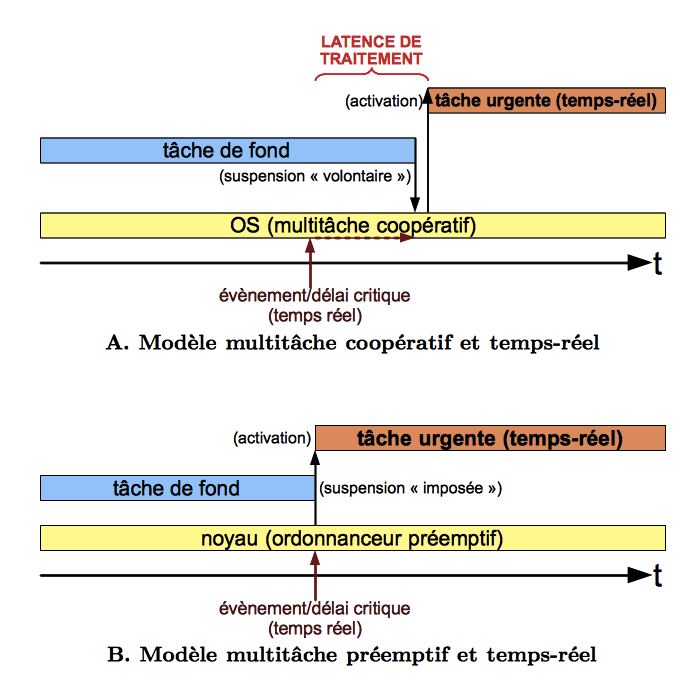
\includegraphics[width=12.75cm]{images/ch3-modeles-multitache.png}
\flcaption{Principe de base du traitement des évènements temps-réel par
les diférents modèles de gestion multi-tâche.}
\label{FigModeleMultitache}
\end{figure}


\subsection{TinyOS}
\label{SubsecTinyOS}

Le premier système ayant connu un large succès dans le domaine des réseaux
de capteurs sans-fil est \nom{TinyOS} \cite{TinyOS}. Il s'agit d'un système
\lang{open-source} et libre (sous license BSD), dont la première version
stable (version 1.0) a été publiée en septembre 2002. Il est extrêmement
léger, et par là-même très bien adapté aux appareils limités que sont
les noeuds des réseaux de capteurs sans-fil de la première génération
(Mica2, MicaZ \cite{DSMicaZ}, TelosB~/ SkyMote \cite{DSTelosB}, etc.).

Ce système a permis de nombreuses avancées dans le domaine, comme la
possibilité d'utiliser le protocole réseau Internet (IP, y compris dans
sa dernière version~: IPv6) ainsi que des protocoles de routage (comme
RPL) sur les réseaux au standard IEEE 802.15.4. Il a également introduit
la possibilité de simuler des réseaux de \lang{motes} fonctionnant sous
TinyOS, grâce au simulateur \nom{TOSSIM} \cite{TOSSIM}.

L'un des principaux défauts de ce système est la nécessité d'apprendre
un langage spécifique~--- nommé \nom{nesC} \cite{nesC}~--- pour pouvoir
travailler et développer des applications avec TinyOS. Contrairement à
ce que son nom pourrait laisser penser, le langage nesC est très différent
du langage C classique et de tous les autres langages informatiques
impératifs couramment utilisés~--- il ressemble plutôt, dans sa philosophie,
aux langages de description de matériel utilisés dans la conception de
circuits intégrés, comme VHDL ou Verilog. En cela, il peut se révéler
difficile à apprendre et à maîtriser pour des programmeurs ayant une
formation de développement informatique classique.

La présence de ce langage spécifique au sein du projet TinyOS n'est pas
un hasard~: TinyOS est en effet construit sur ses propres paradigmes
spécifiques. Ce système gère les entrées~/ sorties (I/O) de façon
totalement asynchrone, et fonctionne autour d'une pile unique, depuis
laquelle les différents composants constituant une application TinyOS
sont appelés en tant que \lang{callbacks} statiquement liés. 
TinyOS a en effet été conçu pour fonctionner de façon principalement
évènementielle, via la programmation de gestionnaires d'interruptions.

La notion de <<~tâche~>> de longue durée existe, mais la gestion du
multitâche est sous TinyOS particulièrement limitée~: les <<~tâches~>>
sont exécutées l'une après l'autre, suivant une file (FIFO) dont l'ordre
ne peut être modifié~--- l'ordonnanceur de TinyOS n'est pas conçu
pour changer dynamiquement l'ordre des tâches à exécuter en fonction
du déroulement de l'application et de son environnement. Les tâches
ne peuvent en outre être préemptées que par des interruptions
(<<~évènements~>>) mais jamais par d'autres tâches. Le manuel
de TinyOS définit en fait les tâches comme des appels de procédures
différés (\lang{``Deferred Procedure Calls''}). Ce fonctionnement
permet toutefois de minimiser grandement la consommation d'énergie,
toute la \lang{mote} étant en sommeil lorsqu'aucune tâche n'a à
s'exécuter (le prochain réveil étant provoqué par <<~l'évènement~>>
suivant).

Il est clair que le fonctionnement de TinyOS et ses paradigmes sont
particulièrement atypiques par rapport aux autres systèmes décrits
dans la présente section. Ceci se ressent dans la programmation
d'applications, qui nécessite de maîtriser ces notions pour savoir
décomposer tout programme en divers <<~évènements~>>, <<~tâches~>> et
autres <<~commandes~>> (appel d'un composant à un autre) pour créer
les composants constituant les applications.
La difficulté d'apprentissage et de maîtrise de ce système pour un
informaticien formé et habitué aux notions classiques de programmation
sera ainsi assez ardue.

L'ensemble des architectures matérielles sur lesquelles TinyOS a été porté
semble actuellement se limiter aux familles AVR et MSP430 (un portage sur
des architectures plus puissantes comme les Cortex-M est évoqué dans la
FAQ du site Web de TinyOS, mais son état d'avancement actuel est inconnu).

Enfin, signalons que TinyOS nécessite l'emploi d'outils de développement
dédiés (langage spécifique oblige) pour pouvoir être compilé.

Toutes ces limitations, ajoutées à un rythme de développement relativement
lent~--- la dernière version stable (2.1.2) remonte à août 2012~--- ont
ces dernières années nui à son adoption, et il n'est désormais plus
le système de référence ni le plus utilisé dans le domaine des réseaux
de capteurs sans-fil.


\subsection{Contiki}
\label{SubsecContikiOS}

Le système d'exploitation de référence dans le domaine des réseaux de
capteurs sans-fil et par extension de l'Internet des objets (IoT) est
\nom{Contiki} \cite{ContikiOS}. Il s'agit également d'un système
\lang{open source} et libre (license BSD), dont la première version
publiée remonte à 2002. Le projet Contiki a été à l'origine de nombreuses
avancées~: on pourra citer entre autres la pile TCP/IP embarquée \nom{uIP}
\cite{uip} depuis étendue en \nom{uIPv6} (qui est présentée comme la pile
IPv6 fonctionnelle la plus légère qui soit), la pile réseau \nom{Rime}
\cite{Rime} simplifiée et orientée vers les économies d'énergie,
ou encore le simulateur avancé de réseaux de capteurs sans-fil
\nom{Cooja} \cite{Cooja}.

S'il est légèrement plus exigeant en ressources que TinyOS, Contiki
reste très léger et particulièrement bien adapté aux \lang{motes}
constituant les réseaux de capteurs sans-fil.

Son principal avantage sur TinyOS est d'être basé sur des paradigmes
standards, avec une API reprenant les principes classiquement rencontrés
dans le domaine des systèmes d'exploitation~; il est en outre codé en
langage C standard~: ceci rend son apprentissage et sa maîtrise bien plus
facile pour un programmeur ayant un cursus classique.

Contiki est basé sur un noyau événementiel, implantant un modèle
multitâche coopératif. Il offre également une pile réseau complète,
directement prête à l'emploi.

Il a été porté sur une multitude de plate-formes, comprenant de nombreuses
\lang{motes} pour réseaux de capteurs sans-fil, mais aussi de vieux modèles
d'ordinateurs personnels~--- Commodore~64, Apple~II, Atari~800XL...~---
et même certains modèles de consoles de jeux (dans des portages
non-officiels).

Des modules optionnels permettent également de fournir des fonctionnalités
aussi diverses qu'une interface graphique, un système de fichiers, ou
encore une mise à jour du programme (\lang{``firmware''}) durant
l'exécution (suivant un processus certes complexe).

Toutes ces caractéristiques et avantages ont largement contribué à la
diffusion et à l'adoption massive de Contiki, ce qui fait qu'il s'agit
désormais du système d'exploitation de référence dans le monde des
réseaux de capteurs sans-fil.

Les développeurs de Contiki ont également été actifs quant au développement
de la couche MAC/RDC~: nombre de protocoles classiques (comme par exemple
X-MAC) ont été implantés dans la pile réseau de ce système~; et un nouveau
protocole, ContikiMAC \cite{ContikiMAC}, a été spécifiquement conçu pour
jouer le rôle de protocole RDC par défaut de Contiki (en collaboration avec
le protocole CSMA/CA du standard IEEE 802.15.4 en tant que couche MAC).
Nous avons abordé ce protocole ContikiMAC dans l'étude des protocoles
LPL plus haut en section \vref{ParContikiMAC}.

Toutefois, la compacité de Contiki, son optimisation et ses fonctionnalités
imposent en contrepartie diverses limitations à ce système.

Contiki est basé sur un modèle multitâche coopératif, et non préemptif~:
l'ordonnanceur de tâches se déclenche en réaction à des <<~évènements~>>
(pour reprendre la terminologie de Contiki). Cet ordonnanceur ne peut se
déclencher que selon un rythme spécifique, dont la fréquence (intervalle
de déclenchement) est déterminée à la compilation. Ce modèle de
fonctionnement multitâche est, comme nous l'avons vu ci-dessus en section
\vref{SubsecMultitache}, un obstacle à la présence de fonctionnalités
temps-réel.

Il faut en outre noter que l'ordonnanceur coopératif de Contiki est
conçu pour traiter un type spécifique de tâches nommé \nom{protothreads}
\cite{Protothreads}. Ce mécanisme permet de gérer différentes files
d'exécution (\lang{``threads''}) sans avoir besoin de maintenir
une pile d'exécution séparée pour chacun d'entre eux.
Le grand avantage de cette technique est la possibilité d'utiliser une pile
unique pour tout un système, diminuant ainsi significativement la quantité
de RAM nécessaire, sans pour autant devoir se limiter à un mécanisme
d'ordonnancement statique comme dans TinyOS.
Ce mécanisme de \lang{protothreads} est d'ailleurs utilisé dans
plusieurs autres applications en dehors de Contiki.
La contrepartie de ce mécanisme est qu'il est nécessaire de respecter
certaines règles rigoureuses quant à l'utilisation de certains éléments
du langage C~: il est notamment impossible d'utiliser l'instruction
\texttt{switch} dans certaines parties d'un programme utilisant ces
\lang{protothreads}.

Toutes ces limitations du système Contiki ont posé des problèmes
non résolus pour nos travaux de thèse, comme nous le verrons dans
la section \vref{SecLimContiki} du présent manuscrit.


\subsection{Nano-RK}
\label{SubsecNanoRK}

Un système spécialisé dans les réseaux de capteurs sans-fil présentant
des propriétés très intéressantes, et surtout proches de nos besoins, est
\nom{Nano-RK} \cite{NanoRK}. Il a été conçu à l'Université de Carnegie
Mellon à partir de 2005.

Il s'agit également d'un système \lang{open source}, publié selon un schéma
de double licence permettant l'utilisation de la GNU GPL (\lang{General
Public License}) si tel est le choix du développeur. On peut donc le
considérer comme un logiciel libre.

Celui-ci fournit de nombreuses fonctionnalités intéressantes~:

\begin{itemize}

\item Un noyau fonctionnant en mode \emph{tickless} (c'est-à-dire sans
nécessiter un \lang{timer} le déclenchant de façon régulière).

\item Un \emph{ordonnanceur temps-réel} avec \emph{multi-tâche préemptif
gérant les priorités}.\\
La granularité théorique~--- permettant de descendre jusqu'à la nano-seconde
par l'utilisation de la représentation temporelle POSIX, réimplantée sous
le nom de \texttt{nrk\_time\_t}~--- est excellente. Mais en pratique, la
granularité effective garantie pour les interruptions (\lang{``timer
tick''}) est de l'ordre de la milliseconde \cite{NanoRKTimeMgt}.
Cela implique une gigue (\lang{``jitter''}) pouvant aller jusqu'à
1000~microsecondes, alors que la durée de base d'une période de
\lang{backoff} CSMA/CA est de seulement 320~microsecondes.
Les fonctionnalités temps-réel de Nano-RK, aussi avancées et complètes
soient-elles, offrent donc une granularité pouvant ne pas être suffisante
pour nos travaux.

\item Un paradigme de \emph{réservations de ressources } très intéressant,
permettant par exemple d'accorder respectivement 100 ms de temps d'exécution
ou l'envoi de 10 paquets par seconde pour une tâche ou un noeud donnés.
Il s'agit en fait d'un principe de quotas, assuré par le noyau système,
et permettant de prévoir un <<~budget énergétique~>> consommé par un
appareil donné pendant une période de temps. Il s'agit d'une spécificité
très avancée et fonctionnellement très prometteuse de Nano-RK.

\item Une occupation mémoire réduite (bien que légèrement supérieure
à celle de TinyOS ou Contiki).

\item Une gestion intégrée des erreurs fatales (violations d'espace
mémoire ou de \lang{timing}, \lang{watchdog}, chutes d'alimentation
énergétique...)

\item Le système est écrit en langage C standard, et est donc compilable
avec le compilateur GNU GCC classique.

\item Une pile réseau légère, comprenant notamment plusieurs protocoles
MAC classiques, dont le protocole LPL B-MAC (voir section
\vref{ParBMAC})~; d'autres protocoles spécifiques et expérimentaux
sont proposés, ainsi qu'une fonction simple de passerelle vers
un réseau IP nommée \lang{``SLIPStream''}.

\end{itemize}

Ce système a le principal désavantage d'avoir été porté sur un nombre limité
d'architectures de microcontrôleurs~: seules les plates-formes MSP430 et AVR
sont supportées, avec une activité et une spécialisation nettement plus
grandes vis-à-vis de cette dernière. Les principales plates-formes
matérielles sur lesquelles Nano-RK est employé sont en effet~:
\begin{itemize}

\item la \lang{``mote''} MICAz \cite{DSMicaZ}, de conception déjà ancienne
(contemporaine de la TelosB/SkyMote) basée sur un MCU ATmega128L
\cite{DSATmega128L} et le classique TI CC2420 \cite{DSCC2420} comme radio~;

\item la plus récente FireFly3 \cite{FireFly3}, spécifiquement conçue
par Carnegie Mellon pour servir de plate-forme matérielle à Nano-RK.
Elle a la particularité d'être conçue autour d'un microcontrôleur intégrant
un émetteur~/ récepteur radio, l'ATmega128RFA1 \cite{DSATmega128RFA1},
et peut accueillir plusieurs cartes d'extension, notamment une carte
comportant de nombreux capteurs (température, pression, humidité,
accéléromètre, audio, mouvement...).

\end{itemize}

Ces deux \lang{``motes''}, mises en avant sur le site de Nano-RK, sont
toutes deux basées sur l'architecture Atmel AVR. Si cela peut présenter
certains avantages~--- comme la possibilité, mise en avant par le projet,
de développer et déboguer directement Nano-RK avec l'outil Atmel Studio~---
cela implique une forte limitation au niveau de la portabilité, laquelle
est pourtant l'un des principaux objectifs recherchés en utilisant un
système d'exploitation pour développer sur WSN.

Aucune activité de portage sur d'autres matériels ou architectures ne
semble entreprise~: cela est fort regrettable, sachant que les
\lang{``motes''} basées sur des microcontrôleurs 32 bits (comme ceux
d'architecture ARM), plus puissantes, apparaissent et se répandent
de plus en plus.

Cela n'empêche toutefois pas Nano-RK d'être encore activement développé
(bien qu'avec des moyens humains visiblement limités, comme beaucoup de
projets strictement académiques), et de faire régulièrement l'objet
de publications, citons par exemple \cite{NanoRKHW2013}.

Toutefois, malgré ces qualités, nous n'avons pas dans le cadre de cette
thèse travaillé avec Nano-RK, car nous avons été amenés à découvrir une
autre plate-forme logicielle très intéressante et plus ouverte.
Nous allons maintenant aborder cette plate-forme dans la section
\ref{SubsecRIOTOS} ci-dessous.


\subsection{RIOT OS}
\label{SubsecRIOTOS}

Nous avons été amenés à nous intéresser, dans le cadre de nos travaux
de thèse, à \nom{RIOT OS} \cite{RIOT}.

Ce nouveau système~--- sa première version a été publiée en 2013~---
est également \lang{open source} et publié sous une licence libre
(LGPL v2.1), et est spécifiquement conçu pour les noeuds de réseaux
de capteurs sans-fil.

Il est développé principalement avec le soutien de la
\lang{Freie Universität Berlin}, de l'INRIA, et de la
\lang{Hamburg University of Applied Sciences}. Il est à noter que
l'équipe de développement de ce projet est particulièrement accueillante
et ouverte aux contributions extérieures.

\medskip

Il fournit les avantages de base que l'on peut attendre d'un OS pour
réseaux de capteurs sans-fil, notamment la portabilité (il fonctionne
sur de nombreux appareils reposant sur les architectures MSP430, AVR et
ARM~--- notamment la famille des Cortex-M), ainsi qu'un ensemble complet
de fonctionnalités, notamment une pile réseau.

Parmi les fonctionnalités offertes, on retrouve de nombreuses capacités
avancées des autres OS spécialisés dans les capteurs sans-fil (comme
Nano-RK), plus d'autres \lang{a priori} inédites~:

\begin{itemize}

\item Un \emph{micro-noyau} léger, dirigé par les interruptions,
fonctionnant par défaut de façon \lang{tickless} (c'est-à-dire sans
nécessiter qu'un \lang{timer} le déclenche de façon régulière).

\item Un ordonnanceur, intégré au micro-noyau, fonctionnant en mode
\emph{multi-tâche préemptif avec gestion des priorités}.

\item Une utilisation optimisée des \emph{timers matériels grâce à une
API dédiée}, permettant de programmer le déclenchement d'actions avec
une granularité très fine, de l'ordre de la dizaine de microsecondes.

\item Des structures de données de base~: piles, files, listes
chaînées et circulaires.

\item Des mécanismes de communication entre tâches (\lang{threads)}~:
notamment un système de passage de messages~--- implanté par l'utilisation
de queues (FIFO) de messages, appartenant chacune à un \lang{thread}
donné~---, ainsi que des \lang{mutex}.

\item RIOT est entièrement écrit en \emph{langage C standard}~;
de plus, contrairement à Contiki, il n'y a aucune restriction quant
aux éléments utilisables du langage (telles que les limitations
imposées par les \lang{protothreads}).

\item Une conception claire et modulaire, rendant le développement
avec mais aussi \emph{dans} le système plus facile et productive.

\item Une gestion des erreurs critiques, que nous avons dans le cadre
de cette thèse initiée et contribué à mettre en place.

\end{itemize}

Les trois premières fonctionnalités citées ci-dessus font de RIOT
un système \emph{temps-réel} à part entière.

\bigskip

Notons que le mécanisme de gestion des \lang{timers} matériels a évolué
pendant l'année 2015. L'ancien mécanisme \texttt{hwtimer}, qui était intégré
au noyau lui-même, a été supprimé et remplacé par un module nommé
\texttt{xtimer}.

Toutes les expériences décrites dans ce manuscrit ont, sauf indication
contraire, été basées sur une version de RIOT utilisant l'ancien système
\texttt{hwtimer} intégré au noyau. Celui-ci a été conçu pour offrir
la possibilité d'utiliser les \lang{timers} matériels du microcontrôleur,
et ce avec une granularité aussi fine que le permettent les \lang{``ticks''}
de ces \lang{timers}. Sur les premières \lang{motes} que nous avons utilisé
(voir section \vref{SecHWMSP430}), nous avons ainsi disposé d'une granularité
d'environ $30,5~\mu$s pour programmer le déclenchement de nos évènements.

\medskip

Le nouveau module \texttt{xtimer} permet lui de s'abstraire de la notion
de \lang{``tick''}, c'est à dire du délai (en général fixe) entre deux
déclenchements successifs d'un \lang{timer} matériel, pour proposer des
délais exprimés systématiquement en microsecondes, le module \texttt{xtimer}
étant conçu pour être implanté sur la base d'un timer matériel dont la
cadence est fixée à 1~MHz. Cette implantation lui permet donc d'atteindre,
en théorie, une granularité à la microseconde près~; dans les faits,
les délais d'exécution des fonctions mêmes de \texttt{xtimer}, ainsi que
la possibilité de préemption par le noyau (hors gestionnaire d'interruption)
génèrent une gigue allant jusqu'à quelques dizaines de microsecondes, soit
(dans les cas les moins favorables) une granularité comparable
à celle offerte par le mécanisme précédent.

Notons quoi qu'il en soit que la disponibilité en standard d'une granularité
temporelle, pour les mécanismes temps-réel de RIOT, de l'ordre de la dizaine
de microsecondes (c'est-à-dire largement inférieure à la milliseconde) 
est une fonctionnalité exceptionnelle~: nous ne l'avons retrouvée lors
de nos recherches dans aucun autre OS dédié aux WSN (par exemple, dans
Nano-RK \cite{NanoRKTimeMgt} qui dispose pourtant d'un mécanisme de
\lang{timing} évolué). Même FreeRTOS (cf. section \vref{SubsecFreeRTOS})
n'offre par défaut qu'un mécanisme de \lang{software timer} d'une granularité
d'1~ms, l'utilisation des potentialités des \lang{timers} matériels étant
laissée à la seule charge du développeur d'applications
\cite{FreeRTOSTimerRes}.

Le fonctionnement \lang{tickless} du noyau et l'utilisation optimale
des \lang{timers} matériels font également de RIOT OS une plate-forme
logicielle prometteuse pour le développement d'applications particulièrement
optimisées et économes en énergie, ces deux fonctionnalités permettant
potentiellement de garder le MCU en état de <<~sommeil~>> (basse
consommation) durant une fraction de temps aussi élevée que possible.
Nano-RK a déjà exploré la piste du fonctionnement \lang{tickless} pour
augmenter son efficacité énergétique (voir \cite{NanoRKTimeMgt}).

\medskip

Un des désavantages de RIOT, par rapport à TinyOS et Contiki, est sa
plus grande exigence en ressources matérielles, notamment concernant
l'occupation mémoire. La pile réseau complète (de la couche physique
à l'implantation 6LoWPAN en passant par les couches RPL et MAC~/ RDC)
ne peut pas être compilée pour un matériel de type SkyMote~/ TelosB
car la quantité de mémoire exigée dépasse celle disponible sur ces
appareils. À l'heure actuelle, des noeuds limités comme ceux basés
sur l'architecture MSP430 sont cantonnés sous RIOT au rôle de RFD,
les rôles de FFD étant pour l'instant réservés aux matériels plus
puissants (comme ceux basés sur des microcontrôleurs ARM).

Notons toutefois que, grâce à l'architecture modulaire du système,
le noyau RIOT compilé avec les seules couches PHY et MAC~/ RDC reste
très léger et occupe très peu de mémoire, étant ainsi parfaitement
compatible même avec les appareils les plus limités. 

En outre, la partie réseau du système ayant fait l'objet d'une
réorganisation en profondeur (comme nous le verrons plus en détail
ultérieurement en section \vref{SecGnrcRIOT}), nous espérons qu'à
l'avenir, il sera possible d'utiliser encore plus efficacement
des appareils aux ressources limitées sous RIOT.

\medskip

Notons également qu'outre la pile réseau intégrée de RIOT, la pile
\nom{OpenWSN} \cite{OpenWSN} a fait l'objet d'un portage sur le noyau
RIOT. Ce dernier est donc l'une des deux plates-formes logicielles
sélectionnées pour accueillir cette pile à hautes performances (l'autre
étant le noyau FreeRTOS \cite{FreeRTOS}). 


\subsection{Autres OS spécialisés}
\label{SubsecAutresOS}

D'autres systèmes d'exploitation spécifiquement conçus pour les réseaux
de capteurs sans-fil ont été développés, mais ceux-ci sont nettement
moins utilisés, et souffrent de limitations nous ayant empêché 
d'envisager sérieusement leur utilisation.

\begin{description}

\item[SOS] \cite{SOS}
Le développement de ce système a été arrêté en novembre 2008. Ses auteurs
recommandent explicitement sur leur site Web de <<~considérer l'utilisation
d'alternatives activement maintenues.~>>

\item[Lorien] \cite{LorienOS}
Si celui-ci est basé sur approche orientée composant intéressante,
ce système ne semble pas d'une utilisation très répandue. Il n'est
actuellement disponible que pour un seul type de matériel (TelosB~/
SkyMote) ce qui limite considérablement la portabilité que l'on est
en droit d'attendre de l'utilisation d'un OS, donc son intérêt.
En outre, son développement semble avoir nettement ralenti,
la dernière version stable publiée par le projet Lorien datant de 2011,
tandis que le dernier \lang{commit} dans le dépôt SourceForge du
projet (r46) remonte à janvier 2013.

\item[Mantis] \cite{MantisOS}
Alors que ce projet prétend être \lang{open source}, celui-ci n'a
publié aucune version accessible sur son site SourceForge~; en outre,
l'accès au dépôt source du projet
(\texttt{http://mantis.cs.colorado.edu/viewcvs}) semble défaillant.
Enfin, les dernières nouvelles officielles affichées sur la page Web
principale du projet parlent d'une version bêta censée être publiée en 2007.
Les dernières publications scientifiques concernant MantisOS semblent
également remonter à l'année 2007. Tous ces éléments nous font penser
que ce projet est tombé à l'abandon...

\item[LiteOS] \cite{LiteOS}
Ce système offre des fonctionnalités très intéressantes, notamment
la possibilité de mettre à jour le \lang{firmware} des noeuds à la
volée, depuis la connexion réseau sans-fil (mise à jour
\lang{``Over-the-Air''}, dont LiteOS semble avoir été le pionnier),
ainsi que le support intégré d'un système de fichiers hiérarchique.
Malheureusement, LiteOS est actuellement uniquement disponible pour
les plates-formes matérielles IRIS et MicaZ, et nécessite l'emploi
d'Atmel Studio pour son développement. Cela nuit gravement à la
portabilité du système, vu que LiteOS semble très fortement lié
à l'architecture de microcontrôleurs AVR.

\item[MansOS] \cite{MansOS}
Ce système très récent offre de nombreuses fonctionnalités
intéressantes, comme le multi-tâche préemptif (de façon optionnelle),
une pile réseau intégrée, et un langage de script. Il est disponible
sur deux architectures de microcontrôleurs~: AVR et MSP430 (mais
malheureusement, pas les architectures ARM dont la progression est
constante). En outre, les capacités temps-réel du système semblent
limitées~: seuls des \lang{timers} logiciels d'une granularité
minimale de 1~milliseconde semblent disponibles.

\item[NanoQplus] \cite{NanoQplus2008}
Il s'agit d'un système dédié aux WSN, apparu semble-t-il en 2008,
annonçant des fonctionnalités intéressantes comme le multitâche
préemptif, une grande portabilité sur de nombreuses architectures de MCUs
(allant des 8~bits aux 32~bits), et surtout un système de protection mémoire.
L'article de 2008 le présentant \cite{NanoQplus2008} semble prometteur, et
un autre article de 2011 \cite{NanoQplusIPv6RPL2011} indique qu'une pile
IPv6 ainsi que RPL y ont été portés.\\
Malheureusement, le site du projet
(\texttt{http://dukemon.tistory.com/tag/NanoQplus}) est exclusivement
en coréen, et seul un faible nombre d'articles écrits en Corée (le plus
souvent en coréen) semblent y faire référence~--- les deux publications
citées dans le présent paragraphe, certes en anglais, sont parues dans
des journaux~/ évènements se voulant internationaux mais s'étant déroulés
en Corée.\\
Il semble donc malheureusement difficile de se faire une idée précise
de ce système, dont l'adoption hors de son pays d'origine semble
actuellement extrêmement limitée.

\item[OpenTag]
Il s'agit d'une pile réseau chargée d'implanter le protocole
DASH7 (standard ISO/IEC 18000-7, spécialisé dans le RFID et incompatible
avec le standard IEEE 802.15.4), fournie avec son propre système
temps-réel minimaliste (noyau dédié). S'il s'agit \lang{stricto sensu}
d'un système fonctionnant sur des WSN, lesdits WSN sont très différents
de ceux que nous étudions dans cette thèse~--- ils fonctionnent par
exemple à la fréquence radio de 433~MHz réservée à DASH7. Leur
développement a au départ été prévu pour des applications militaires.
Il ne s'agit donc pas d'un système comparable à tous ceux que nous
avons vu jusqu'à présent, et ne correspond absolument pas aux travaux
de notre thèse.

\end{description}


\subsection{OS temps-réel classiques~/ généralistes}
\label{SubsecOSTempsReel}

Une autre possibilité utilisée par plusieurs constructeurs de
\lang{motes} est de recourir à des systèmes embarqués <<~classiques~>>,
lesquels offrent le plus souvent des fonctionnalités temps-réel.

\subsubsection{FreeRTOS}
\label{SubsecFreeRTOS}

\hyphenation{Free-RTOS}

La référence actuelle en matière de système d'exploitation temps-réel
\lang{open source} pour l'embarqué est \nom{FreeRTOS} \cite{FreeRTOS}.

FreeRTOS est un projet mature (première version publiée en 2003),
stable et très largement employé, notamment dans l'industrie.

Il a été porté sur plus de 30 architectures de microcontrôleurs différentes,
c'est-à-dire quasiment toutes les architectures présentes sur le marché~;
ce qui en fait le système le plus portable cité jusqu'ici dans le présent
manuscrit, largement devant n'importe quel système dédié aux réseaux de
capteurs sans-fil.

L'un des points forts majeurs de FreeRTOS est son excellente documentation~:
le code source est abondamment et consciencieusement commenté, et l'auteur
publie deux manuels complets (en anglais uniquement) sur son système~:
\begin{enumerate}
\item un manuel d'utilisation \cite{FreeRTOSTuto}, complet et très
didactique, tant sur l'utilisation du système lui-même que sur les notions
de temps-réel en informatique et les conséquences de ces notions quant aux
bonnes pratiques de programmation~;
\item un manuel de référence du système \cite{FreeRTOSRef}, détaillant
de façon exhaustive l'API et les options de configuration, avec de
nombreux exemples de code (\lang{``listings''}).
\end{enumerate}
Ces deux ouvrages, rédigés avec soin et maintenus à jour, facilitent
considérablement l'apprentissage et la programmation avec ce système.
Il s'agit également d'une des sources de revenus du projet FreeRTOS,
ces deux manuels étant vendus sous forme électronique sur le site
Web du projet~: cette documentation sur FreeRTOS n'est donc
\emph{pas} libre, contrairement au système lui-même qui est publié
sous la licence GNU GPL.

Le code source du noyau en lui-même se compose uniquement de quatre fichiers
source en langage C~--- dont un représente une fonction optionnelle
(coroutines). Le reste du source du projet se compose des portages (couches
d'abstraction) pour les nombreuses plates-formes matérielles et compilateurs
supportés, et d'exemples. Ce système reste ainsi très léger quant aux
ressources matérielles exigées (généralement moins de 10~Ko de code
programme) ce qui le rend parfaitement adapté aux systèmes embarqués
les plus limités.

La simplicité du noyau (quantité de code minimale) et les critères de
qualité stricts imposés au code source contribuent à la robustesse
de FreeRTOS.

Cela lui permet d'ailleurs de fournir une version certifiée
pour les utilisations dans les systèmes embarqués critiques, nommée
\nom{SafeRTOS}. Contrairement au noyau FreeRTOS de base, SafeRTOS
n'est \emph{pas} un logiciel libre~: l'achat d'une licence payante est
exigé, en échange de la certification (IEC 61508: SIL 3) et d'un support
technique avancé. Cette version spéciale, SafeRTOS, est une autre source de
revenus du projet FreeRTOS (en plus de la vente de manuels citée plus haut).

Citons également l'existence d'\nom{OpenRTOS}, qui est un clone absolu
de FreeRTOS sous une licence \emph{propriétaire}, vendu à l'intention des
industriels rebutés par les exigences de la GNU GPL, et fournissant
également un support technique~--- et par la même occasion une troisième
source de revenus au projet FreeRTOS.

\medskip

Le noyau FreeRTOS fournit des fonctionnalités avancées telles que~:
\begin{itemize}
\item le multi-tâche, préemptif par défaut, coopératif en option,
via un ordonnanceur gérant les priorités~;
\item un mode \lang{``tickless''} optionnel~;
\item des structures de données de base (listes, files)~;
\item des mécanismes de communication entre tâches (\lang{``Inter Process
Communication''})~: sémaphores, \lang{mutex}~;
\item des \lang{timers} logiciels~;
\item et une gestion optionnelle de l'allocation de mémoire
(\lang{``heap''})~: trois mécanismes différents disponibles.
\end{itemize}

Cette compacité a toutefois un prix~: FreeRTOS n'est en fait qu'un
noyau, fournissant les fonctionnalités de base citées ci-dessus.
Il est dépourvu de tout pilote matériel, y compris pour les périphériques
de base intégrés aux microcontrôleurs (par exemple~: les ports séries ou
les GPIO)~--- ces pilotes de périphériques devant être développés et
fournis en sus par les fournisseurs de matériels et~/ ou d'applications
désireux de l'utiliser.

Par conséquent, il est également évident que FreeRTOS ne fournit aucune
pile réseau, aussi rudimentaire soit-elle.

Notons qu'il existe des extensions réseau proposées en sus pour FreeRTOS,
mais la plupart sont des composants logiciels propriétaires et à source
secret (proposés dans le cadre du projet <<~FreeRTOS plus~>>, un écosystème
de logiciels basé sur FreeRTOS), ce qui ne peut convenir pour nos
travaux de thèse.

Toutefois, cette situation pourrait changer, car la pile réseau avancée
\nom{OpenWSN} \cite{OpenWSN} a été développée en prenant pour l'un de ses
noyaux de base FreeRTOS (l'autre noyau étant celui de RIOT OS comme nous
l'avons vu plus haut). Si l'intégration d'OpenWSN et du noyau FreeRTOS
se développe et est amenée à être largement adoptée, nous pourrons alors
compter sur un nouveau système dédié aux réseaux de capteurs sans-fil
à part entière, \lang{open source} et très performant.

\bigskip

Certains constructeurs de capteurs sans-fil ont bâti leur propre système
d'exploitation dédié en se basant sur FreeRTOS~: on pourra notamment citer
la société HiKoB et son projet OpenLab. Malheureusement, un tel projet est
par définition intimement lié à un type de matériel donné, et fait donc
perdre l'un des principaux avantages liés à l'utilisation d'un OS,
à savoir la portabilité.

\subsubsection{Autres OS temps-réel}
\label{SubsecAutresRTOS}

Notons qu'il existe d'autres systèmes temps-réel embarqués et \lang{open
source}, tel qu'\nom{Erika Entreprise}, largement utilisé dans l'industrie
notamment automobile. Ce système, ayant un long historique (première
version datant de 2002), et ayant reçu une certification (OSEK/VDX),
a lui aussi été porté sur de nombreuses plates-formes, dont des \lang{motes}
comme la MicaZ. Toutefois, les WSN ne sont absolument pas la spécialité
de ce système~--- il n'offre aucune pile réseau~---, et s'il a un succès
certain dans l'industrie, il est totalement ignoré dans le milieu de
la recherche académique (nous n'avons trouvé aucune publication le
mettant en {\oe}uvre).

De nombreux autres systèmes d'exploitation temps-réel existent, dotés
d'une licence libre ou propriétaire~--- la plupart du temps destinés
à l'embarqué~---, mais à notre connaissance, aucun d'entre eux n'est
employé, même de façon ponctuelle, dans le cadre des WSN.

\bigskip

FreeRTOS est actuellement l'OS temps-réel embarqué <<~généraliste~>> ayant
largement le plus de succès comme plate-forme de recherche dans le domaine
des réseaux de capteurs sans-fil.


\subsection{Discussion~: les systèmes d'exploitation dédiés}
\label{SubsecDiscussOS}

Depuis l'an 2000, plusieurs OS \lang{open source} spécialisés dans les
réseaux de capteurs sans-fil ont été développés~: TinyOS en a été le
pionnier. Toutefois, ses nombreuses et importantes limitations,
ses paradigmes inhabituels et son langage spécifique inhabituel (nesC)
en font désormais un système en perte d'influence.

\bigskip

La référence actuelle en ce domaine est Contiki~: sa légèreté quant aux
ressources matérielles demandées, ses nombreuses fonctionnalités, assurées
par diverses innovations techniques significatives, l'importante
communauté de développeurs qu'il a su réunir autour de lui, et désormais
le support professionnel assuré par une société fondée par les créateurs
du système (Thingsquare) en font le système incontournable et la référence
dans le domaine des réseaux de capteurs sans-fil.

Celui-ci souffre toutefois de limitations~--- principalement liées aux
choix techniques effectués lors de sa conception, notamment pour créer
un système économe en ressources matérielles.

\medskip

La communauté académique n'en est pas restée là, et a démarré plusieurs
autres projets de systèmes dédiés aux réseaux de capteurs sans-fil. Si
nombre d'entre eux semblent être tombés en désuétude, plusieurs projets
ont montré des qualités dignes d'intérêt~: citons notamment LiteOS,
ayant développé la notion de mise à jour du \lang{firmware} des noeuds
à l'exécution via la communication sur le réseau (\lang{``On the Air''}),
et surtout Nano-RK et RIOT OS, qui sont à la fois des systèmes embarqués
temps-réel \emph{et} conçus pour les réseaux de capteurs sans-fil.

On citera également les OS embarqués <<~classiques~>>, dont FreeRTOS
qui est la référence actuelle en matière de système temps-réel \lang{open
source}. FreeRTOS, comme RIOT, sont les deux noyaux systèmes sélectionnés
pour accueillir la pile réseau avancée OpenWSN, développée pour
implanter l'état de l'art en matière de réseaux de capteurs sans-fil
(notamment les avancées de l'amendement 802.15.4e et la pile protocolaire
6TiSCH).

La liste des principaux OS utilisables pour les réseaux de capteurs
sans-fil, avec leurs points forts et leurs faiblesses, peut ainsi être
résumée dans les données de la table \vref{TblOSWSN}.

\begin{sidewaystable}[!p]
\centering

{\footnotesize
\begin{tabular}{p{18mm}|p{18mm}|p{18mm}|p{20mm}|p{30mm}|p{35mm}|p{20mm}|p{18mm}}
\hline
\textbf{Nom} & \textbf{Noyau}
             & \textbf{Exigences}
             & \textbf{Pile réseau}
             & \multicolumn{2}{p{65mm}|}{\textbf{Fonctionnalités}}
             & \textbf{Portabilité}
             & \textbf{Adoption} \\

             & \textbf{(capacités)}
             & \textbf{matérielles}
             &
             & \textbf{de base}
             & \textbf{spécifiques}
             & \\
\hline
\hline
 \textbf{TinyOS} & modulaire statique &
                   minimales &
                   oui (intégrée) &
                   gestion asynchrone des E/S &
                   langage spécifique (nesC),
                   simili-<<~mode \lang{tickless}~>> &
                   moyenne (AVR, MSP430) &
                   Pionnier, Répandu (mais en baisse) \\
\hline
 \textbf{Contiki OS} & multitâche coopératif &
                       très modérées &
                       deux~: uIPv6 ou Rime &
                       gestion des E/S, \lang{timers} logiciels, 
                       IPC (limitées) &
                       noyau évènementiel, protothreads,
                       reprogrammation à l'exécution &
                       élevée (AVR, MSP430, PIC, etc.) &
                       Très répandu (OS de référence) \\
\hline
 \textbf{Nano-RK} & multitâche préemptif temps-réel &
                    relativement modérées &
                    oui (intégrée) &
                    gestion des E/S, \lang{timers} logiciels, IPC &
                    gestion des erreurs fatales,
                    mécanisme de réservation de ressources,
                    mode \lang{tickless} &
                    assez faible (MSP430 mais surtout AVR) &
                    Relativement répandu \\
\hline
 \textbf{RIOT OS} & multitâche préemptif temps-réel &
                    moyennes (modérées pour le seul noyau) &
                    oui (intégrée), plus utilisation possible
                    d'OpenWSN (projet externe) &
                    gestion des E/S, \lang{timers} logiciels, IPC,
                    structures de données (listes...) &
                    gestion des erreurs fatales,
                    gestion avancée des timers matériels,
                    reprogrammation à l'exécution en cours de développement,
                    mode \lang{tickless} &
                    bonne (MSP430, ARM, AVR, x86) &
                    Moyennement répandu (en expansion) \\
\hline
 \textbf{Lite OS} & multitâche préemptif & 
                    modérées &
                    oui (intégrée) &
                    gestion des E/S, mutex &
                    reprogrammation à l'exécution (pionnier),
                    système de fichiers intégré,
                    journalisation d'évènements &
                    faible (AVR uniquement) &
                    Relativement répandu \\
\hline
 \textbf{Mans OS} & multitâche préemptif en option &
                    relativement modérées &
                    deux~: intégrée et uIPv6 &
                    gestion des E/S, \lang{timers} logiciels,
                    mutex &
                    gestion du GPS,
                    reprogrammation à l'exécution,
                    langage de script disponible &
                    moyenne (AVR et MSP430) &
                    Apparemment peu répandu \\
\hline
\hline
 \textbf{FreeRTOS} & multitâche préemptif temps-réel
                     (coopératif en option) &
                     modérées &
                     non (utilisation possible
                     d'OpenWSN, projet externe) &
                     \lang{timers} logiciels, IPC,
                     coroutines (option),
                     structures de données (listes...) &
                     noyau uniquement, excellente documentation,
                     gestion mémoire,
                     mode \lang{tickless} optionnel &
                     excellente (plus de 35 architectures
                     matérielles) &
                     Extrêmement répandu (généraliste,
                     non dédié aux WSN) \\ 
\hline
\end{tabular}
} %% de footnotesize

\flcaption{Principales plates-formes logicielles utilisables en 2015
dans le cadre des réseaux de capteurs sans-fil.}
\label{TblOSWSN}
\end{sidewaystable}

\bigskip

Ainsi, si Contiki est à l'heure actuelle la référence en matière de
système pour réseaux de capteurs sans-fil, les récentes avancées apportées
par l'amendement 802.15.4e au protocole IEEE pourraient faire évoluer le
paysage.

En effet, l'absence de fonctionnalités temps-réel de Contiki rendent
impossibles les synchronisations temporelles~--- plus exactement~:
le déclenchement d'évènements à des moments extrêmement précis, jusqu'à
quelques dizaines de microsecondes près~--- nécessaires au caractère
\lang{``slotté''} (TDMA et même FDMA) de la nouvelle couche MAC étendue.

Dans ces conditions, le domaine des plates-formes logicielles pour réseaux
de capteurs sans-fil pourrait largement évoluer, et permettre à des
systèmes comme RIOT OS et~/ ou le couple FreeRTOS~/ OpenWSN de
s'imposer à l'avenir dans le paysage des WSN.

\bigskip

Pour les besoins de développement rapide, facile, permettant de passer
facilement de l'émulation au test sur matériel de prototypage, une solution
originale comme \nom{OpenWiNo} \cite{WiNo2013}, qui n'est pas un OS complet,
mais un noyau ultra-léger offrant une pile protocolaire et des
fonctionnalités de gestion de \lang{timers}, pourrait devenir une
alternative intéressante lorsqu'elle sera publiquement disponible.

%%%%%%%%%%%%%%%%%%%%%%%%%%%%%%%%%%%%%%%%%%%%%%%%%%%%%%%%%%%%%%%%%%%%%%%%%%%%%

\section{Conclusion~: protocoles MAC~/ RDC et OS spécialisés}
\label{SecConcluChEtatArt}

L'analyse de l'état de l'art sur les protocoles MAC basés sur la couche
physique du standard IEEE 802.15.4 d'une part, et d'autre part sur les
systèmes d'exploitation dédiés aux réseaux de capteurs sans-fil, nous
permet de faire le lien entre ces deux sujets.

Ainsi, nous pouvons déterminer que pour réussir à implanter efficacement
des protocoles MAC avancés permettant d'optimiser à la fois la qualité
de service <<~fonctionnelle~>> et la consommation d'énergie (voir
\vref{SubsecProtoMACavances}), nous avons besoin de fonctionnalités
temps-réel permettant de réagir efficacement aux évènements, notamment
temporels~--- en d'autres termes, respecter des délais très stricts~---
ces protocoles avancés nécessitant une synchronisation précise entre
les différents noeuds communicants, et souvent un recours au multiplexage
temporel (TDMA), comme iQueue-MAC, ou même la couche MAC du standard
802.15.4 en <<~mode \lang{``beacon''}~>>, \lang{a fortiori} la couche
MAC améliorée de l'extension 802.15.4e.

C'est pourquoi nous chercherons, dans le chapitre \ref{ChPFLogicielles}
suivant, la meilleure plate-forme logicielle (c-à-d. système d'exploitation)
pour atteindre ces objectifs.


%%%%%%%%%%%%%%%%%%%%%%%%%%%%%%%%%%%%%%%%%%%%%%%%%%%%%%%%%%%%%%%%%%%%%%%%%%%%%
%%%                    FIN DU CHAPITRE "ÉTAT DE L'ART"                    %%%
%%%%%%%%%%%%%%%%%%%%%%%%%%%%%%%%%%%%%%%%%%%%%%%%%%%%%%%%%%%%%%%%%%%%%%%%%%%%%


